\subsection{Performance in $\Bs\to\phi\g$ decay}

The decay channel of $\Bs\to\phi\gamma$ is studied with different \ecal cell size configration or luminosity condition. 
In the reconstruction,
the $\phi$ paritcle information is obtained from generated samples.
%thus, 
%we can study the \ecal effect to the decay reconstruction independently.
%the true $\phi$ decayed from $\Bs$ is used in the reconstruction.
Thus, 
the final performance is only related to the different configuration of \ecal in simulation.
Table.~\ref{tab:ecal_bs2PhiGamma} lists all selections used in this channel reconstruction,
the transverse energy of reconstructed gamma is larger than $2600\mev$ and the transverse of the $\Bs$ candidates greater than $3000\mev$.
%$\Delta_{T}$ is the time difference between measured cluster time and the hypothesized time of \g decayed from the $\phi$ vertex.    
%And ${\rm Dis\_track}$, ${\rm PID\_g\_piz}$ and ${\rm PID\_g\_conta}$ are cluster identification variables,
%which have been discussed in Section.~\ref{subsec:ecal_identification}.
Table.~\ref{tab:ecal_bs2PhiGamma} lists the selection applied to the simulation samples,
we name them basic selections here.

\begin{table}[tbh]
\caption{Selection criteria in $\Bs\to\phi\g$ channel.}
\centering
\begin{tabular}{rl}
\hline
Quantity               	& Selections \\
\hline
\pt of \g           	& $>2.6 \gev$ \\
\pt of \Bs			& $>3.0 \gev$ \\
\hline
%$\Delta_{T}$   		& $<$ \\
%\hline
%${\rm Dis\_track}$	& $>20 \mm$ ($>5 \mm$ for small cell size sample)\\
%${\rm PID\_g\_piz}$     & $>$ \\
%${\rm PID\_g\_conta}$   & $>$ \\
%\hline
\end{tabular}
\label{tab:ecal_bs2PhiGamma}
\end{table}

\subsubsection{Luminosity effect}

As mentioned above, 
the luminosity will increase markedly after \upgradetwo,  
the physical performances in this channel with different luminosities are studied first.
20000 simulation samples for each luminosities were generated by this parameterized simulation tool,
and by the way,
the current \ecal cell segmentation is used for these samples.
Figure.~\ref{fig:bs_phiGamma_diff_lumi} shows the $\phi\g$ invariant mass distribution with different luminosities. 
$\lum=4\times10^{32}\cm^{-2}\sec^{-2}$ is the instananeous luminosity during Run 1 and Run 2 at \lhcb, 
and this value can reach up to $\lum=1.5\times10^{34}\cm^{-2}\cdot\sec^{-1}$ after \upgradetwo.
Two other luminosity cases are also studied,
since the instananeous luminosity descends as time goes by in one beam injection, 


%%%%%%%%%%%%%%%%%%%%%%%%%%%%%%%%%%%%%%%%
\begin{figure}[!htb]
  \begin{center}
    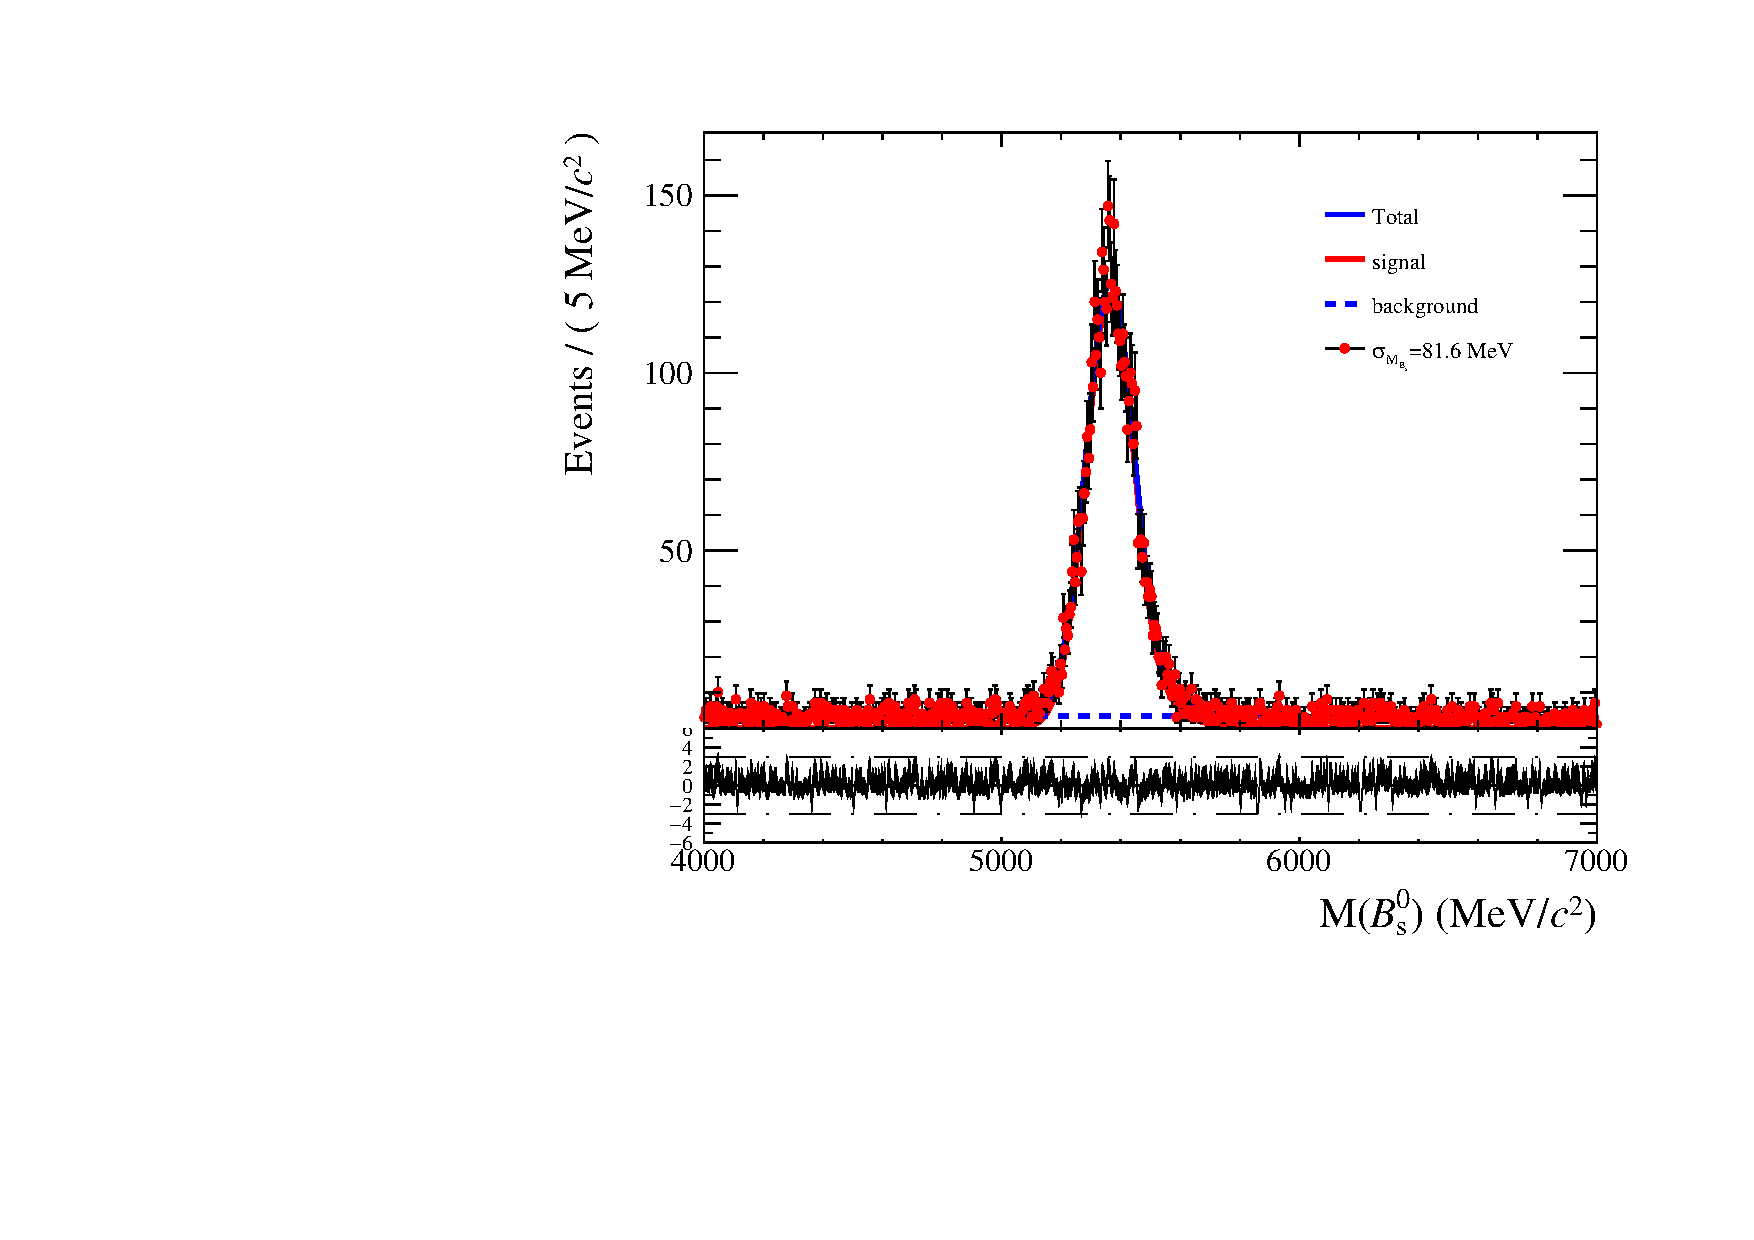
\includegraphics[width=0.45\linewidth]{Figures/06_ECAL/Fast_sim_Bs_PhiGamma/plots/Bs_Big_cell_Lumi_10_32_4.pdf}
    \put(-130,146) {\textrm{\small $\lum=4\times10^{32}\cm^{-2}\cdot\sec^{-1}$}}
    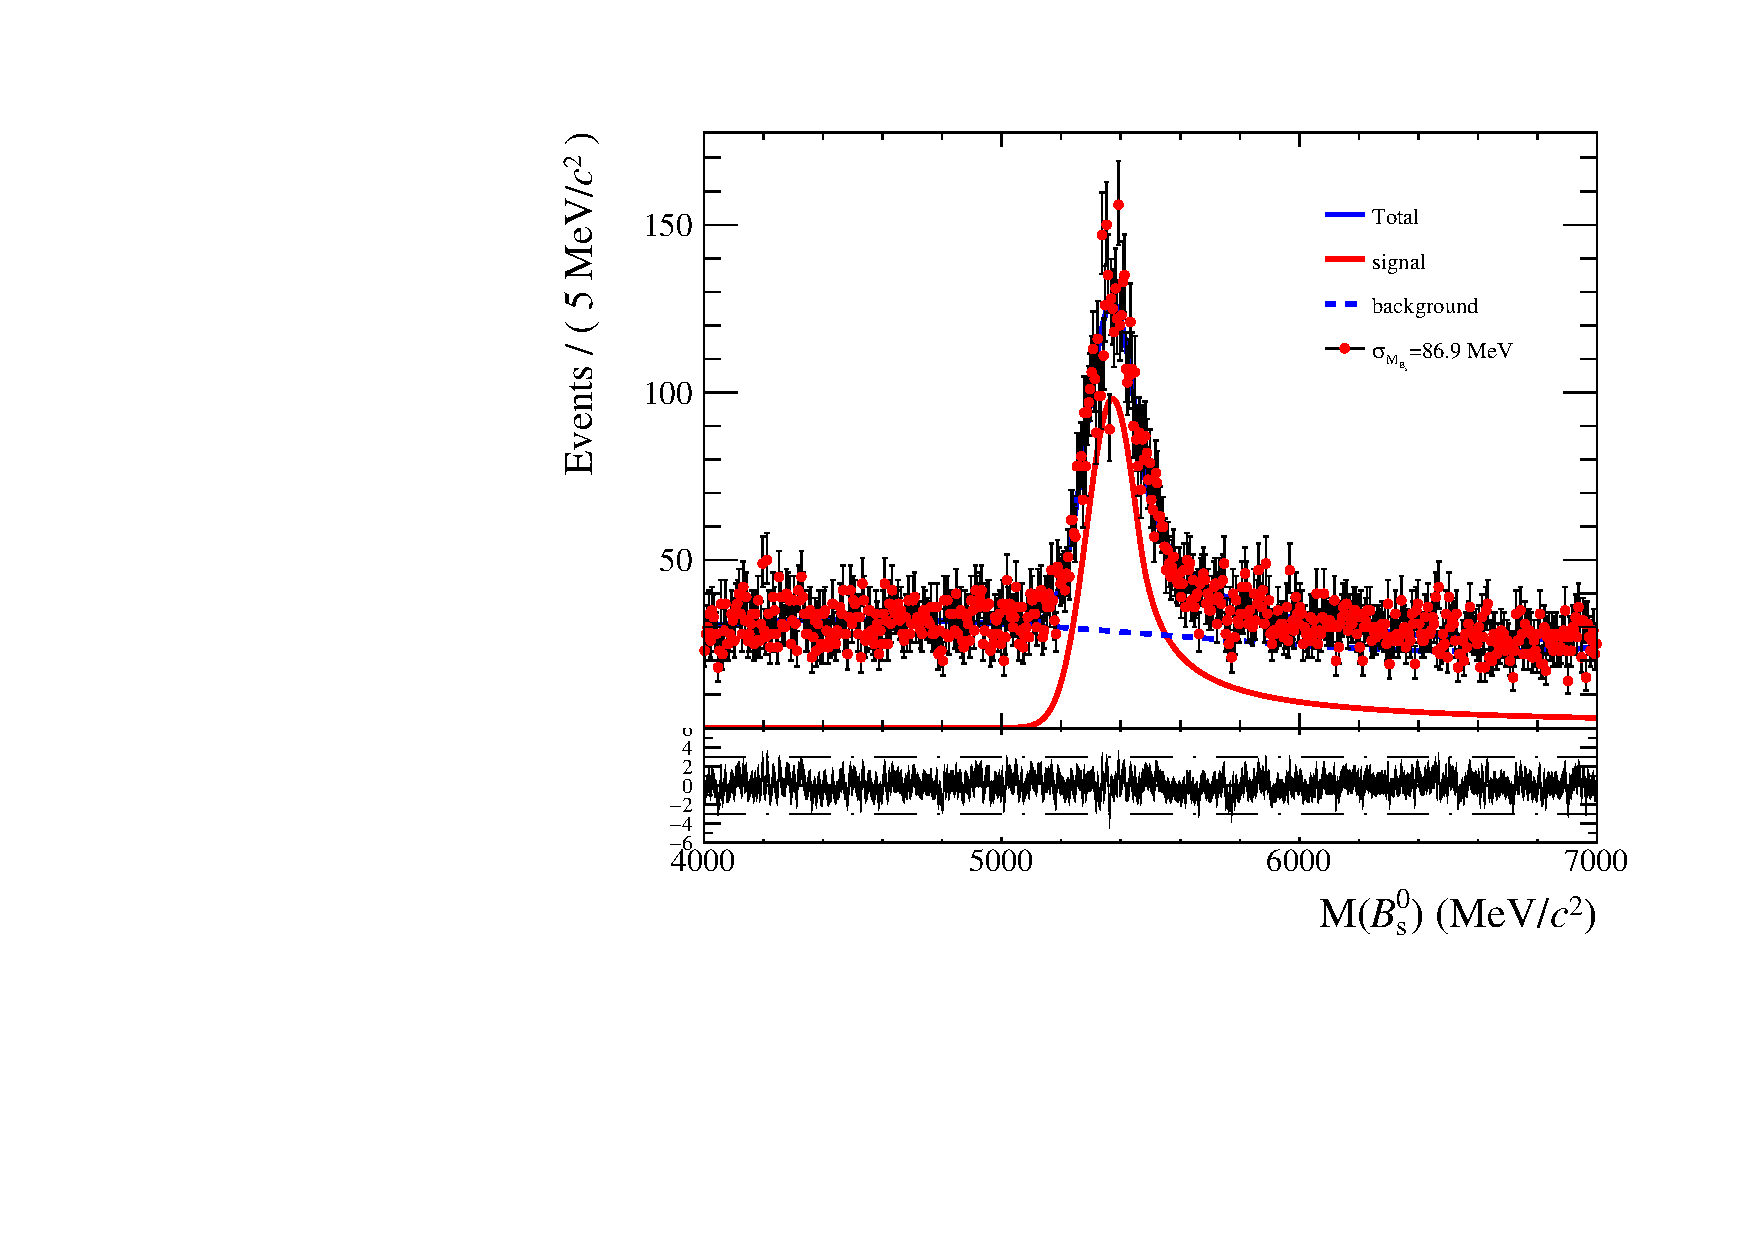
\includegraphics[width=0.45\linewidth]{Figures/06_ECAL/Fast_sim_Bs_PhiGamma/plots/Bs_Big_cell_Lumi_10_33_6.pdf}
    \put(-130,146) {\textrm{\small $\lum=0.6\times10^{34}\cm^{-2}\cdot\sec^{-1}$}}
    \\ 
    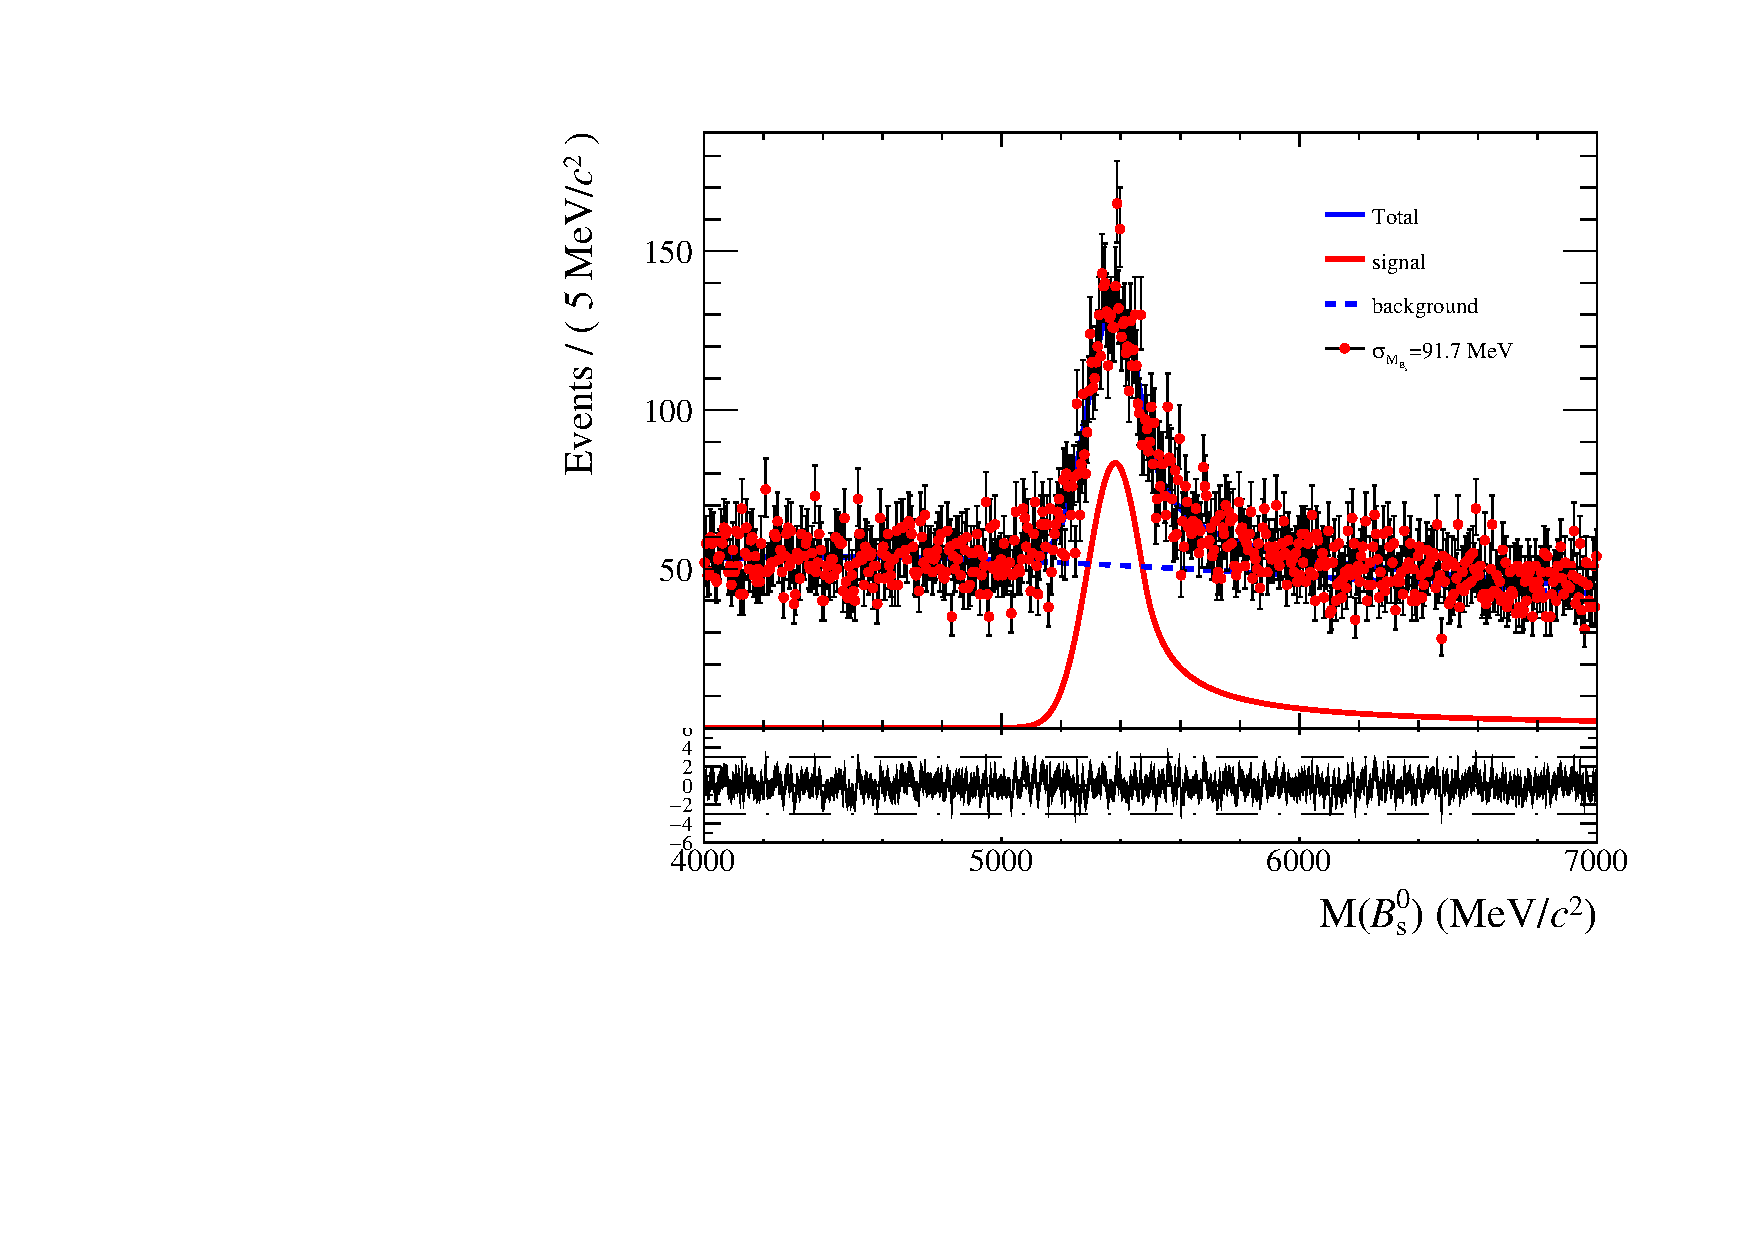
\includegraphics[width=0.45\linewidth]{Figures/06_ECAL/Fast_sim_Bs_PhiGamma/plots/Bs_Big_cell_Lumi_10_33_10.pdf} 
    \put(-130,146) {\textrm{\small $\lum=1.0\times10^{34}\cm^{-2}\cdot\sec^{-1}$}}
    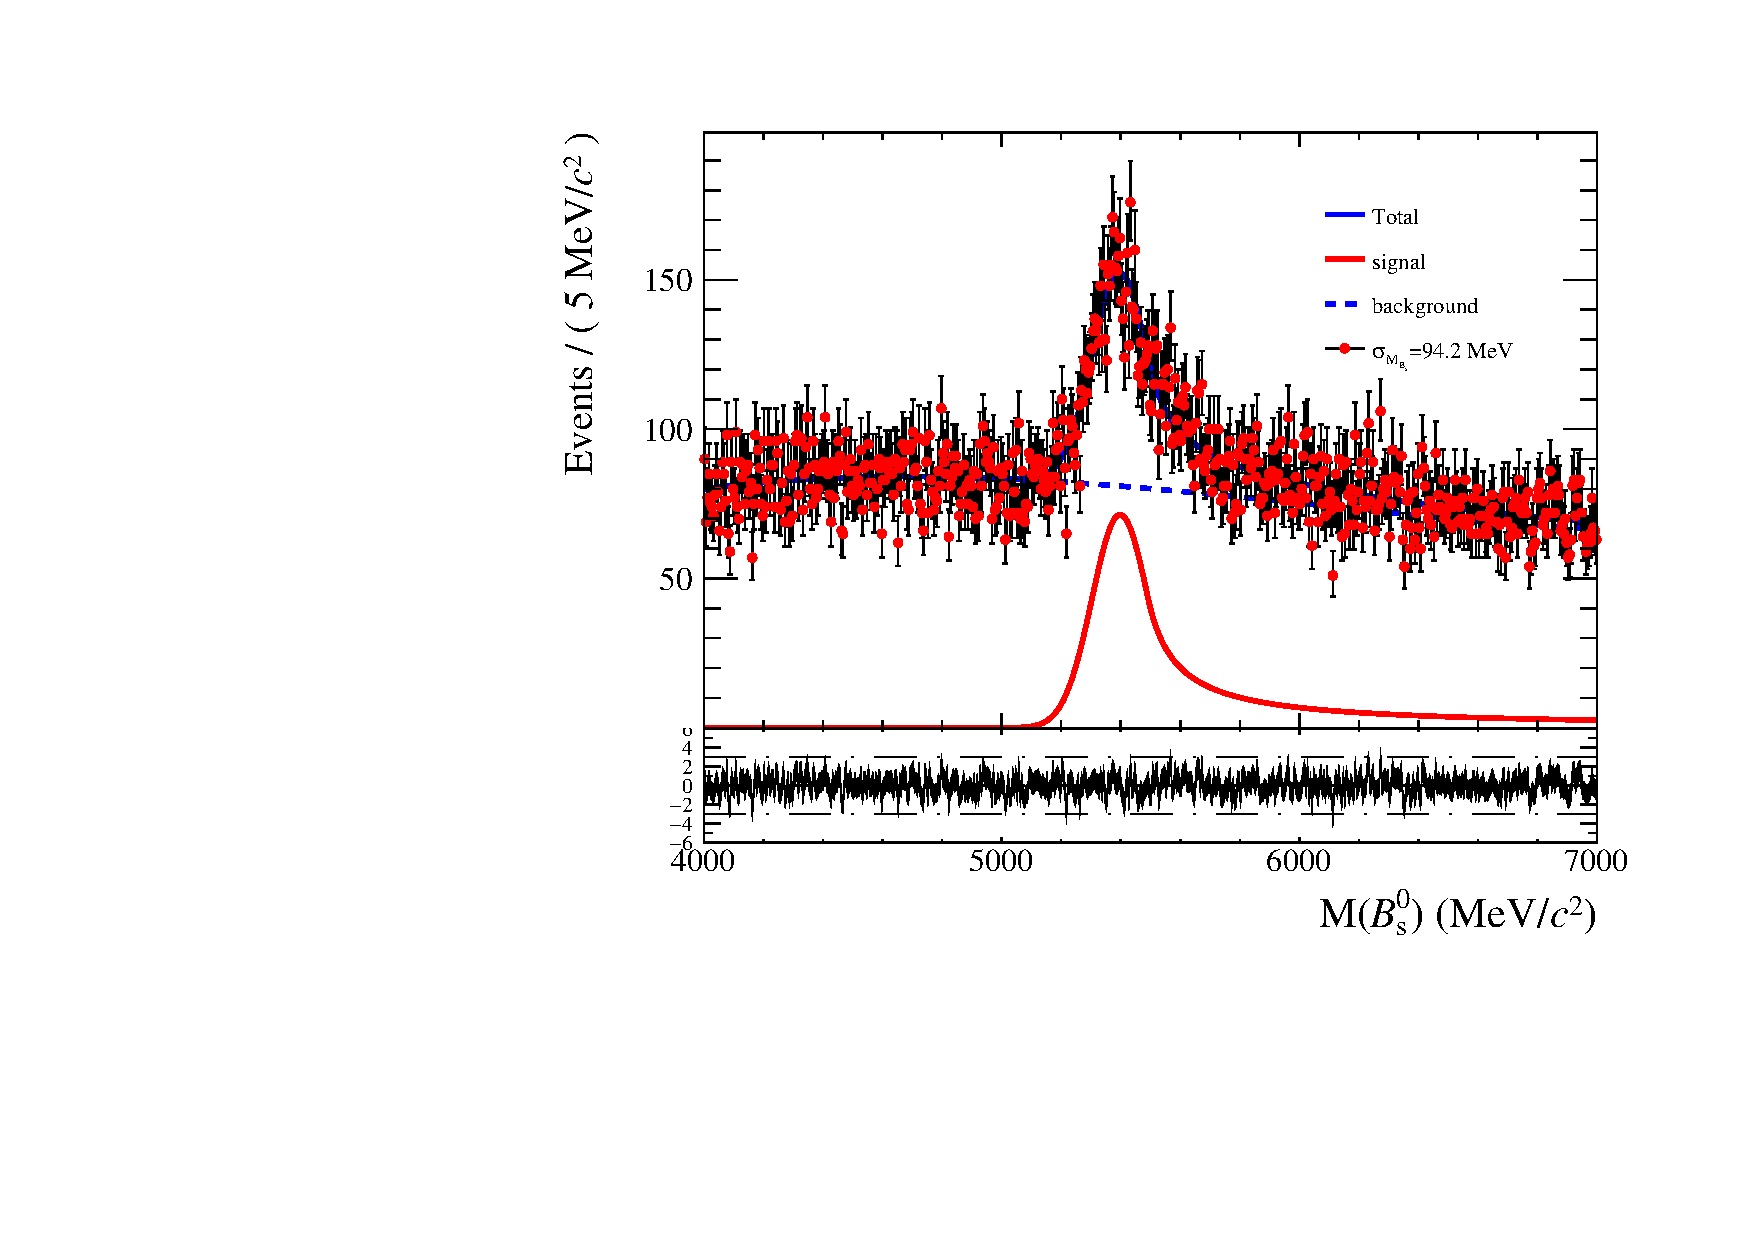
\includegraphics[width=0.45\linewidth]{Figures/06_ECAL/Fast_sim_Bs_PhiGamma/plots/Bs_Big_cell_Lumi_10_33_15.pdf}
    \put(-130,146) {\textrm{\small $\lum=1.5\times10^{34}\cm^{-2}\cdot\sec^{-1}$}}
    \\ 
    \vspace*{-0.5cm}
  \end{center}
  \caption{
  The mass distribution of $\Bs$ in $\Bs\to\phi\g$ decay with different luminosities.
  }
  \label{fig:bs_phiGamma_diff_lumi}
\end{figure}
%%%%%%%%%%%%%%%%%%%%%%%%%%%%%%%%%%%%%%%%

The yields of signal and background are estimated by fitting the mass distribution for each smaple,
where the crystal ball function is used to describe the shape of signal and the background is described 3 order chebyshev polynomial function.
The fitting results are listed in Table.~\ref{tab:ecal_bs2PhiGamma_diff_lumi}.
Comparing these four plots,
the distinguishing feature is 
that the yields of combinatorial background increases rapidly along with the increase of luminosity,
and we found that this increase is linear roughly.
In addition, 
the significance
is deminished due to the high-background.
By the way,
the significance is defined as $S/\sqrt{S+5\dot B}$ here.
The backgound yield is multiplied with a factor of 5 as this value is underestimated from simulation sample,
and this factor was obtained by comparing to previous study\supercite{LHCb-PAPER-2012-042}. 

Besides,
the mass resolution of \Bs becomes larger with luminosity increased.
Most clearly,
a long tail appears in \Bs mass distribution in high luminosity case due to overlapping effect.
Thus,
we need to improve the properties of \ecal to meet these challenges.


\subsubsection{Smaller cell size to remove overlapping effect}

In order to remove the overlapping clusters, 
two other cell size segmentations are studied in parameterized simulation.
The first one is designed according to the rediation\footnote{This configuration was proposed by Philipp Roloff for \lhcb.},
as shown in Figure.~\ref{fig:Phillip_segmentation}.
The other one is very high granularity silicon-tungsten \ecal,
all cells are squares with width equal to $1\cm$,
as shown in Figure.~\ref{fig:geometrySiW}.

%%%%%%%%%%%%%%%%%%%%%%%%%%%%%%%%%%%%%%%%
\begin{figure}[!htb]
  \begin{center}
    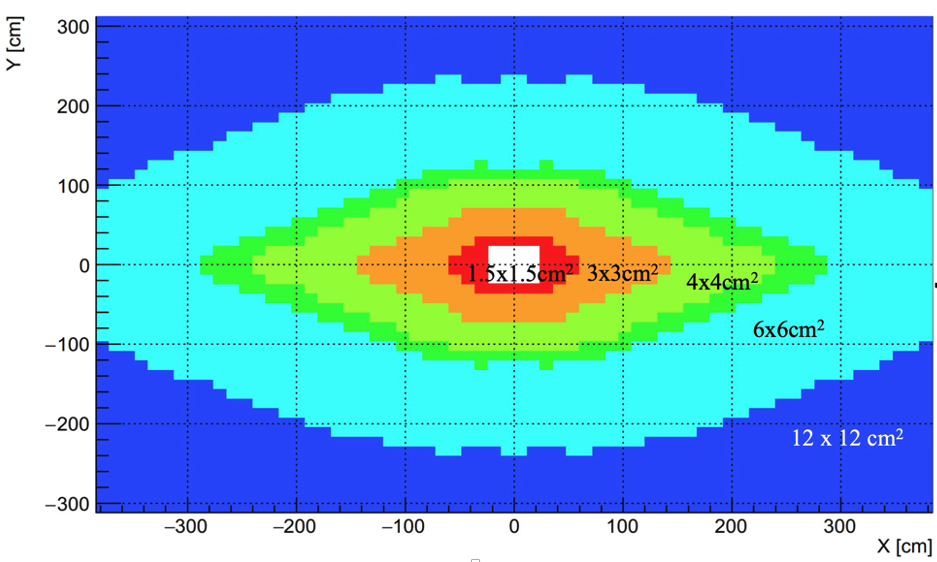
\includegraphics[width=0.55\linewidth]{Figures/06_ECAL/Fast_sim_Bs_PhiGamma/Phillip_segmentation.png}
    \vspace*{-0.5cm}
  \end{center}
  \caption{
  The diagram of \ecal cell size segmentation proposed by Phillip Roloff for \lhcb.
  }
  \label{fig:Phillip_segmentation}
\end{figure}
%%%%%%%%%%%%%%%%%%%%%%%%%%%%%%%%%%%%%%%%


\begin{table}[!tbh]
\caption{The physical performance in different luminosities with different \ecal cell segmentation.}
\centering
\begin{tabular}{ c | c c c c c}
\hline\hline
   Segmentation 
   & \tabincell{c}{Luminosity \\ ($\cm^{-2}\cdot\sec^{-1}$) } 
   %& \tabincell{c}{(-19.37,\\+9.53  )}
   & Efficiency	
   & \tabincell{c}{Bkg \\ ($\times1000$)	}	
   & Significance	
   & \tabincell{c}{Mass resolution \\ (\mev) } \\
\hline
\multirow{4}{*}{Current} &
$4\times10^{32}$           		& $0.25$		& $1.9$	     & $62$		    & $82$ \\
\cline{2-6} &
$0.6\times10^{34}$			& $0.23$ 		& $16.6$         & $33$            & $87$ \\
\cline{2-6} &
$1.0\times10^{34}$			& $0.21$ 		& $29.8$         & $23$            & $92$ \\
\cline{2-6} &
$1.5\times10^{34}$			& $0.19$ 		& $46.7$         & $17$            & $94$ \\
\hline
\multirow{4}{*}{Phillip's} &
$4\times10^{32}$           		& $0.25$		& $1.6$		& $61$		& $109$ \\
\cline{2-6} &
$0.6\times10^{34}$			& $0.23$ 		& $13.9$         & $33$            & $104$ \\
\cline{2-6} &
$1.0\times10^{34}$			& $0.21$ 		& $22.4$         & $24$            & $105$ \\
\cline{2-6} &
$1.5\times10^{34}$			& $0.21$ 		& $31.1$         & $22$            & $105$ \\
\hline
\multirow{4}{*}{Si-W} &
$4\times10^{32}$           		& $0.28$		& $1.8$		& $62$		& $89$ \\
\cline{2-6} &
$0.6\times10^{34}$			& $0.27$ 		& $15.5$         & $38$            & $90$ \\
\cline{2-6} &
$1.0\times10^{34}$			& $0.27$ 		& $22.8$         & $35$            & $85$ \\
\cline{2-6} &
$1.5\times10^{34}$			& $0.24$ 		& $30.2$         & $27$            & $88$ \\
\hline
\hline
\end{tabular}
\label{tab:ecal_bs2PhiGamma_diff_lumi}
\end{table}

In these parameterized simulations,
the energy resolution of Phillip's segmentation is set to be $\sigma(E)/E=0.1/\sqrt{E}\oplus0.024$
\footnote{According to \geant simulation of spaghetti \ecal from other colleagures in \lhcb.}, 
while the energy resolution of Si-W \ecal is $\sigma(E)/E=0.2/\sqrt{E}\oplus0.007$
\footnote{Obtained from \geant simulation of Si-W, details are shown in next section.}.
All results with different simulation configurations are summaried in Table.~\ref{tab:ecal_bs2PhiGamma_diff_lumi}.
According to these simulation samples,
we find that the reconstruction efficiencies do not change significantly.
The significance of smaller cell size is a little better than the value obtained from current segmentation.
Most obviously, 
the number of background candidates becomes larger with higher luminosity. 
%due a better mass resolution.
%Besides,
%the overlapping effect is removed with smaller cell size segmentations,
%as shown in Figure.~\ref{fig:bs_phiGamma_high_lumi_phillip_small}, 
%the long tail in $\Bs$ mass distribution has been removed when comparing to Figure.~\ref{fig:bs_phiGamma_diff_lumi}.

%%%%%%%%%%%%%%%%%%%%%%%%%%%%%%%%%%%%%%%%%
%\begin{figure}[!htb]
%  \begin{center}
%    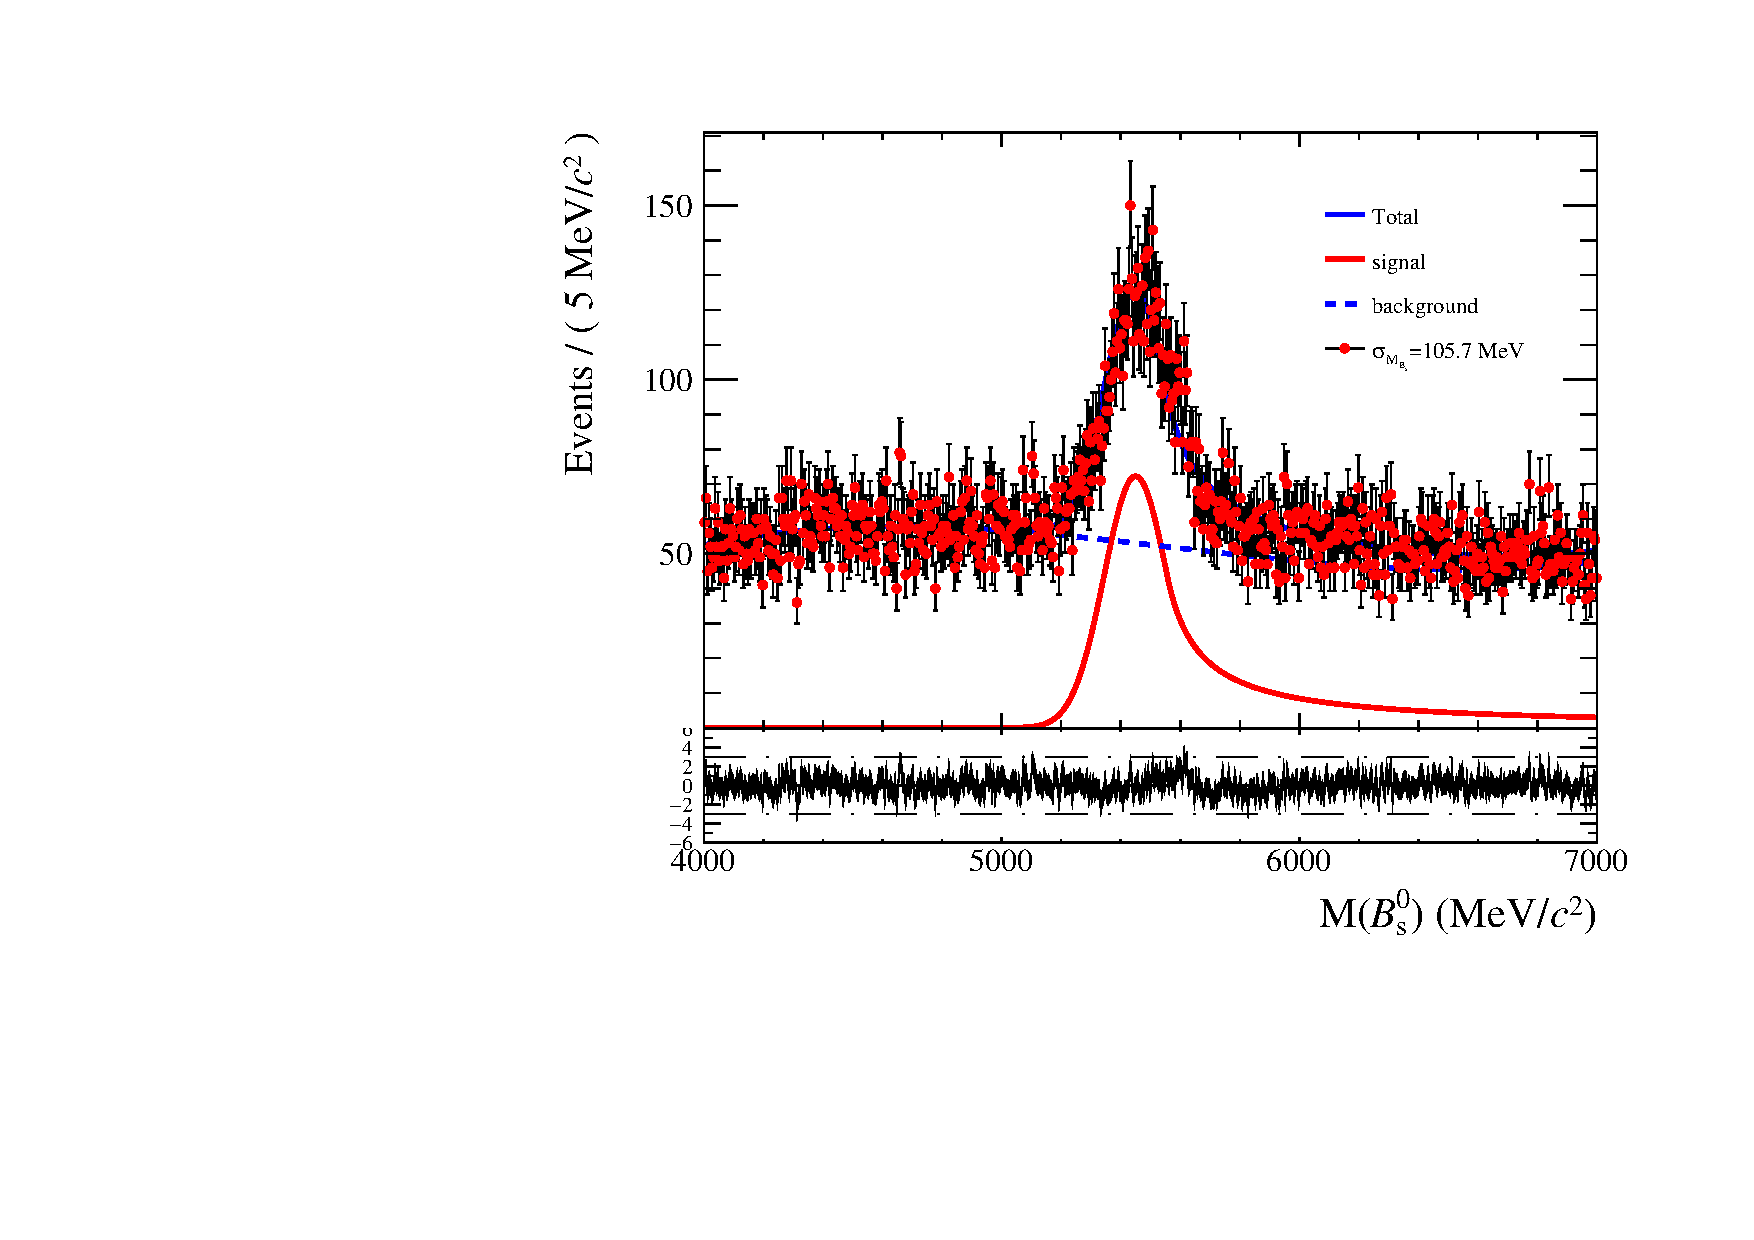
\includegraphics[width=0.45\linewidth]{Figures/06_ECAL/Fast_sim_Bs_PhiGamma/plots/Bs_Phillip_cell_Lumi_10_33_15.pdf}
%    %\put(-130,146) {\textrm{\small $\lum=4\times10^{32}\cm^{-2}\sec^{-2}$}}
%    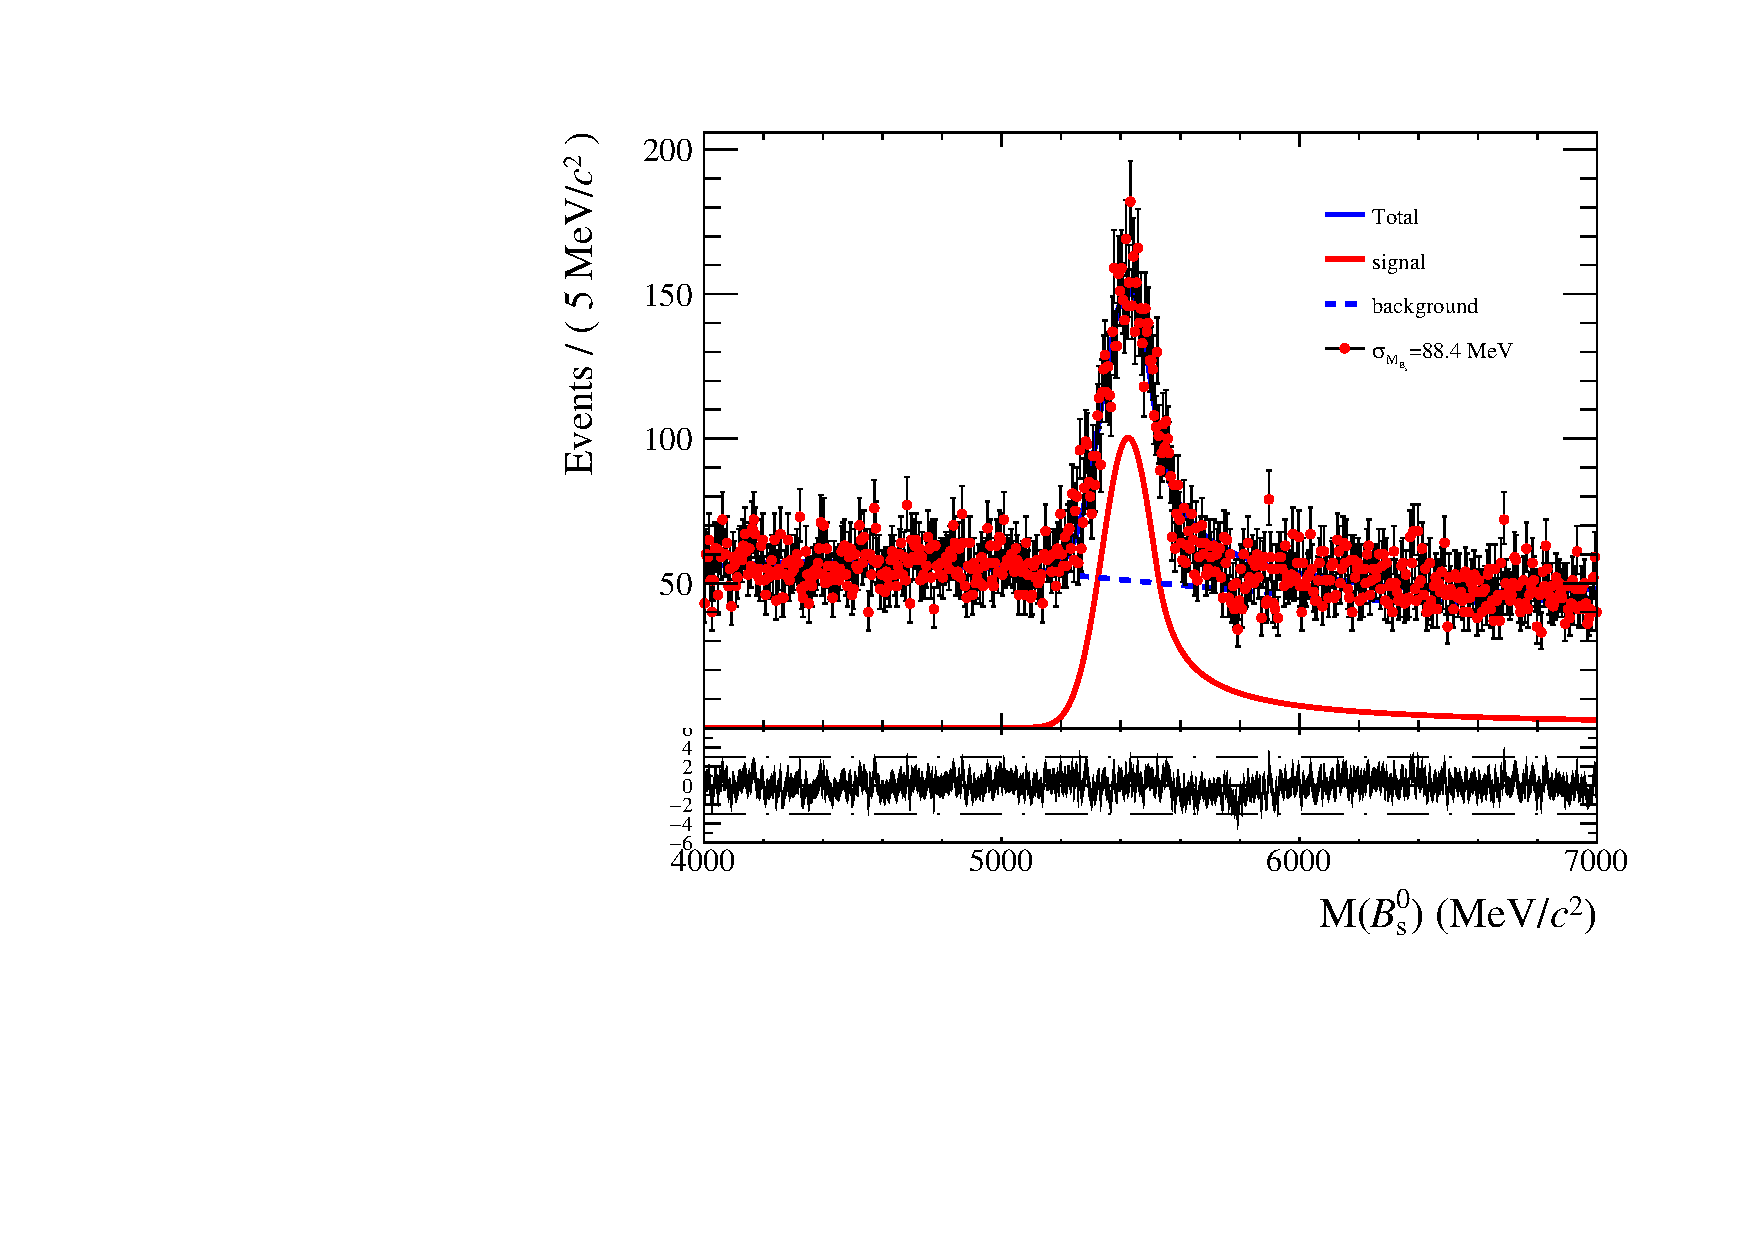
\includegraphics[width=0.45\linewidth]{Figures/06_ECAL/Fast_sim_Bs_PhiGamma/plots/Bs_Small_cell_Lumi_10_33_15.pdf}
%    %\put(-130,146) {\textrm{\small $\lum=0.6\times10^{34}\cm^{-2}\sec^{-2}$}}
%    \\ 
%    \vspace*{-0.5cm}
%  \end{center}
%  \caption{
%  The mass distribution of $\Bs$ in $\Bs\to\phi\g$ decay with luminosity equal to $\lum=1.5\times10^{34}\cm^{-2}\cdot\sec^{-1}$,
%   the left one represents Phillip's segmentation, right one represents Si-W segmentation.
%  }
%  \label{fig:bs_phiGamma_high_lumi_phillip_small}
%\end{figure}
%%%%%%%%%%%%%%%%%%%%%%%%%%%%%%%%%%%%%%%%%


\subsubsection{Precision timing to remove pile-up effect}

%%%%%%%%%%%%%%%%%%%%%%%%%%%%%%%%%%%%%%%%
\begin{figure}[!htb]
  \begin{center}
    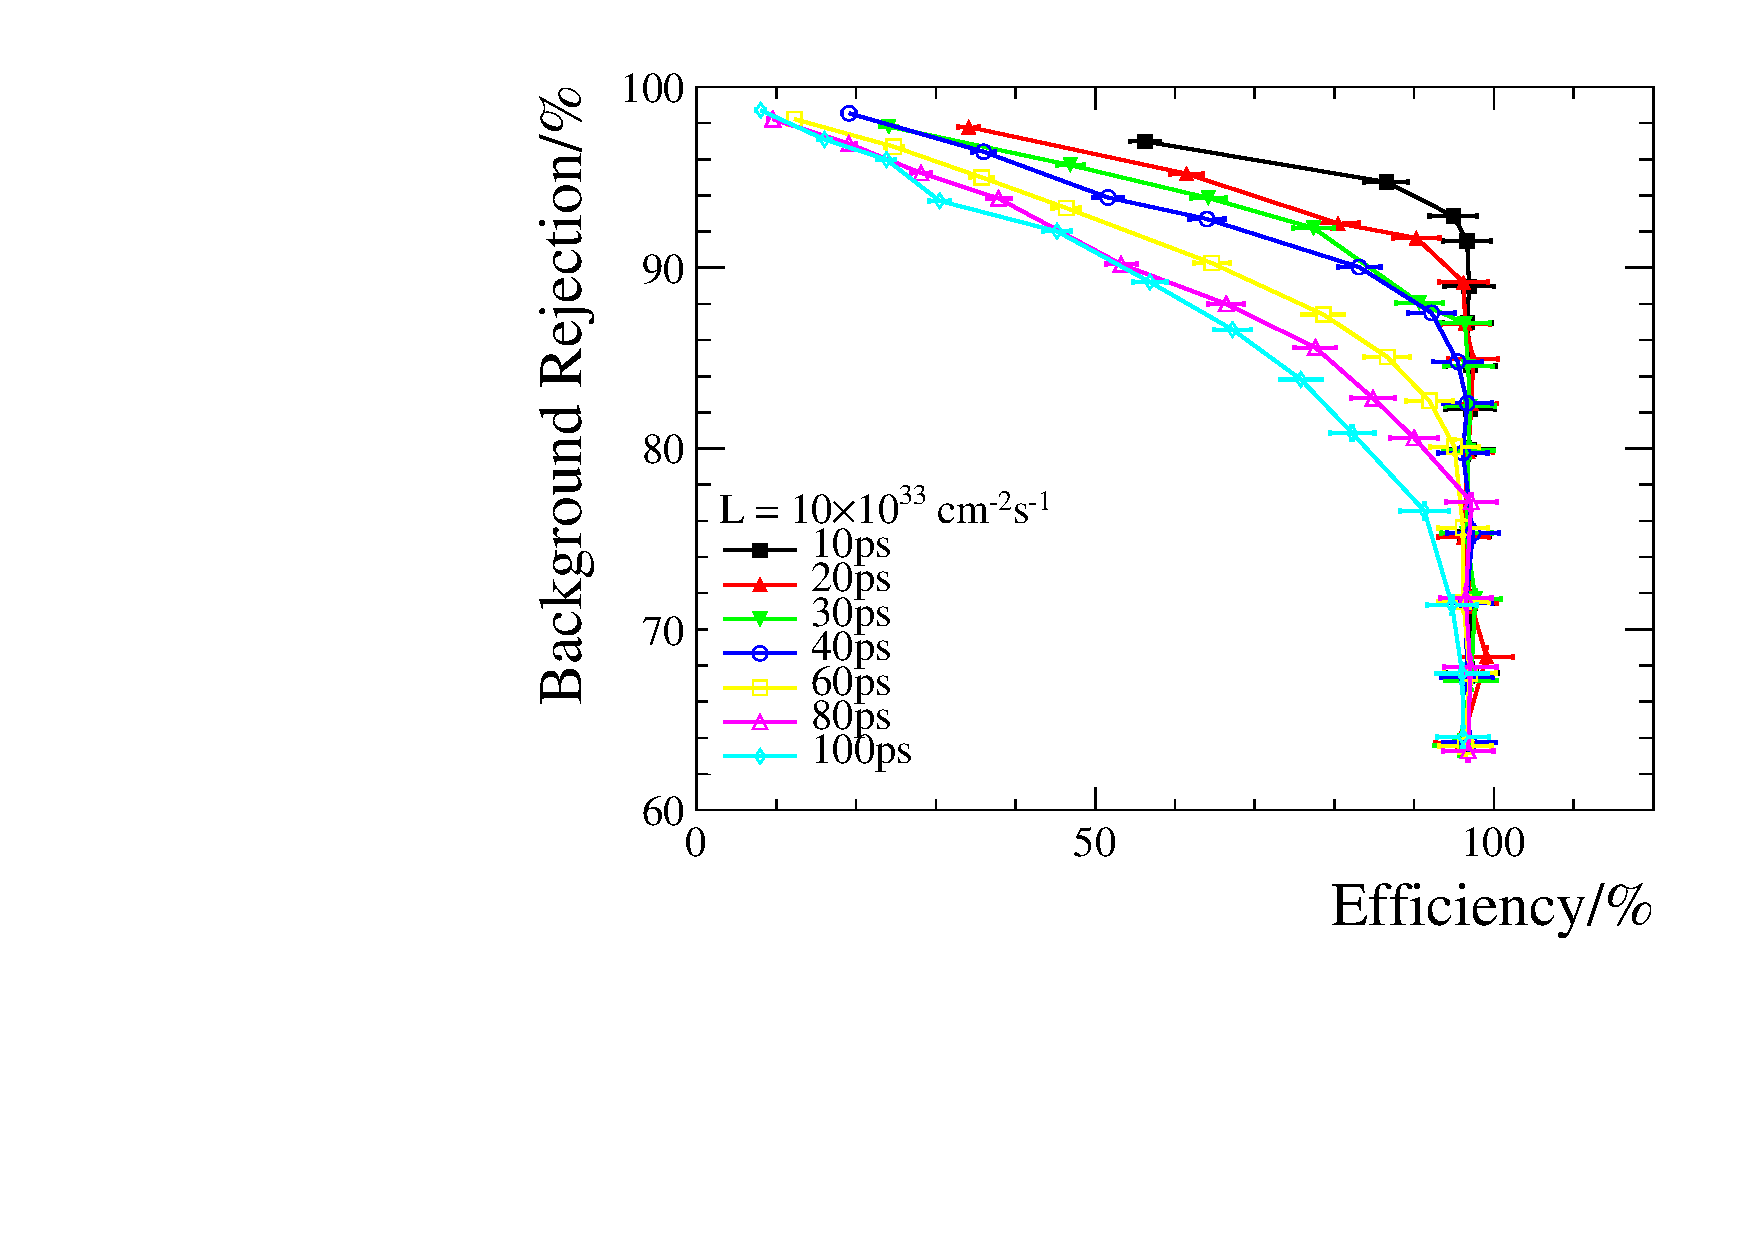
\includegraphics[width=0.45\linewidth]{Figures/06_ECAL/Fast_sim_Bs_PhiGamma/eff_vs_other/eff_vs_rej_Phillip_cell_Lumi_10_33_10.pdf} 
    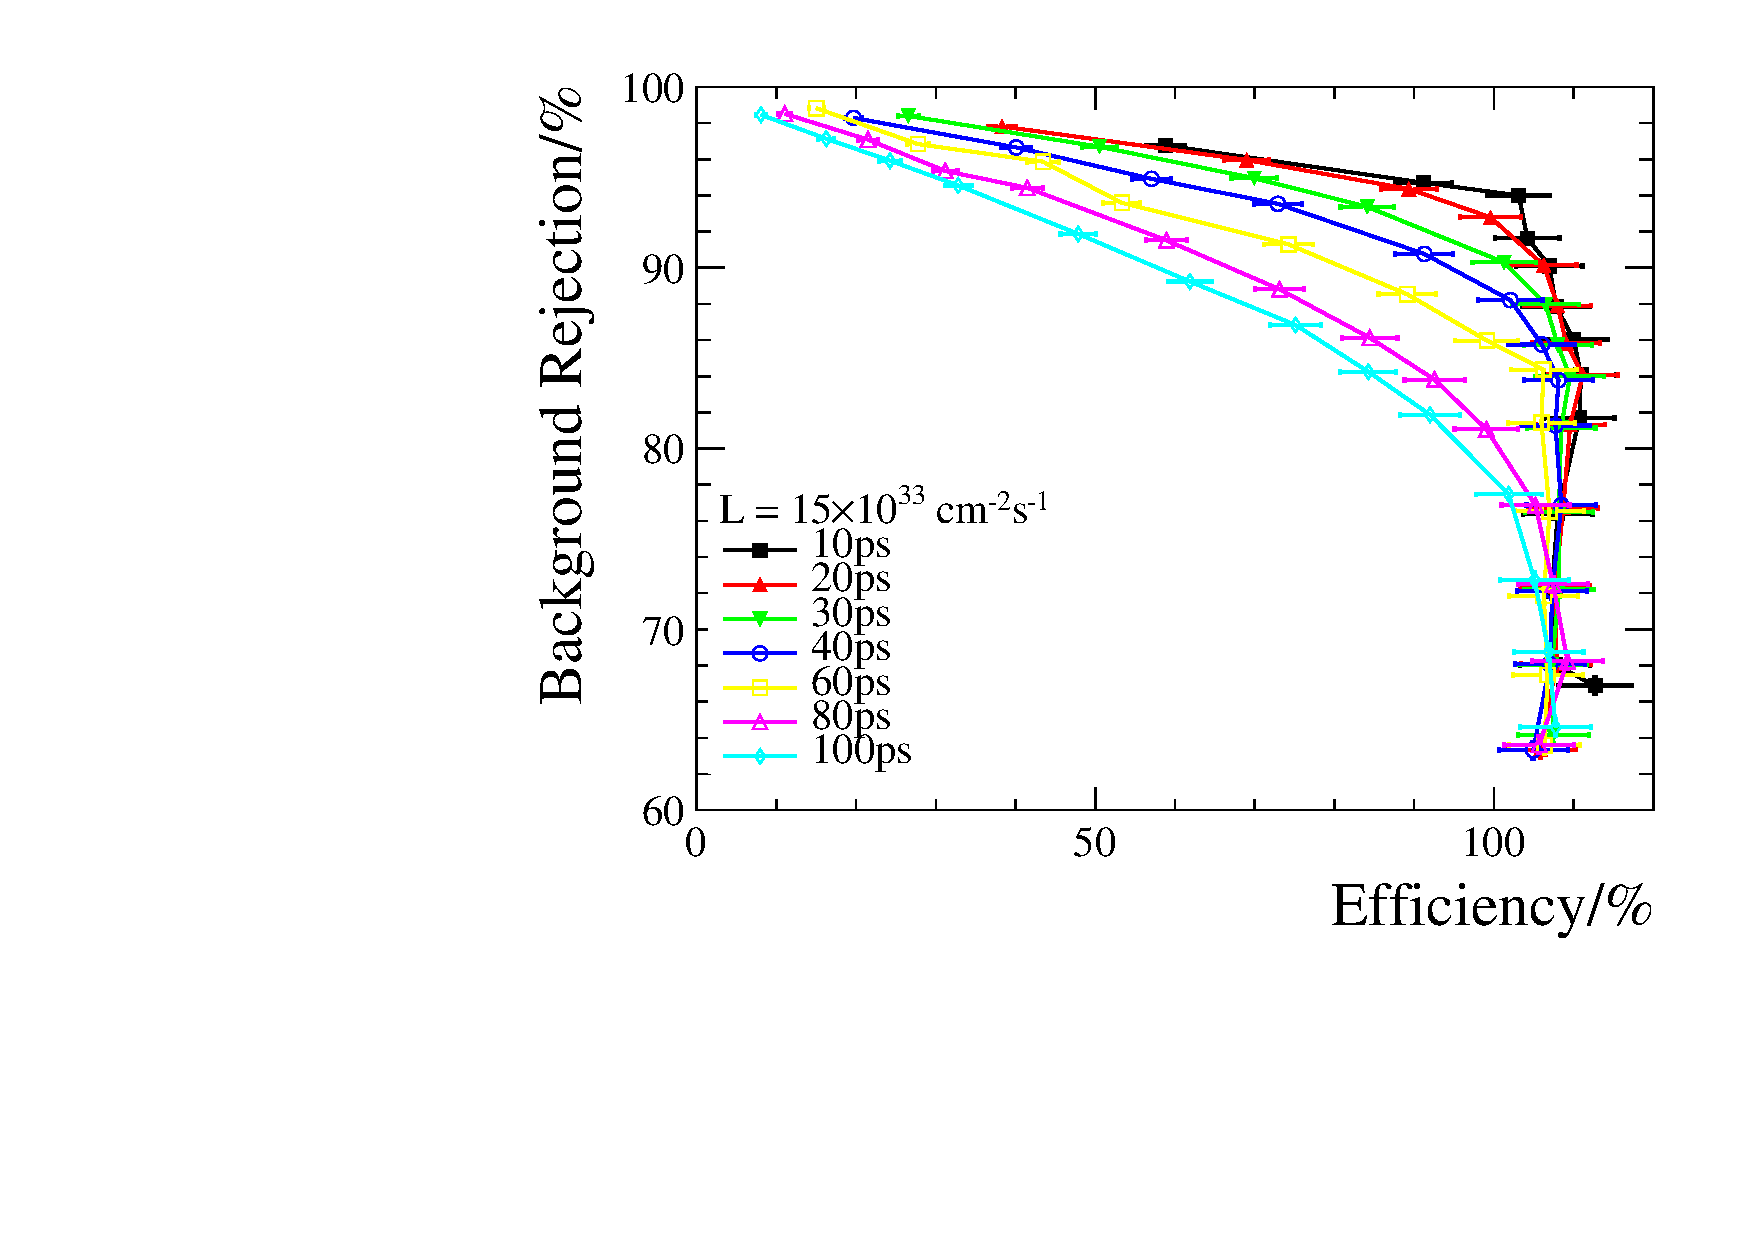
\includegraphics[width=0.45\linewidth]{Figures/06_ECAL/Fast_sim_Bs_PhiGamma/eff_vs_other/eff_vs_rej_Phillip_cell_Lumi_10_33_15.pdf}
    \\ 
    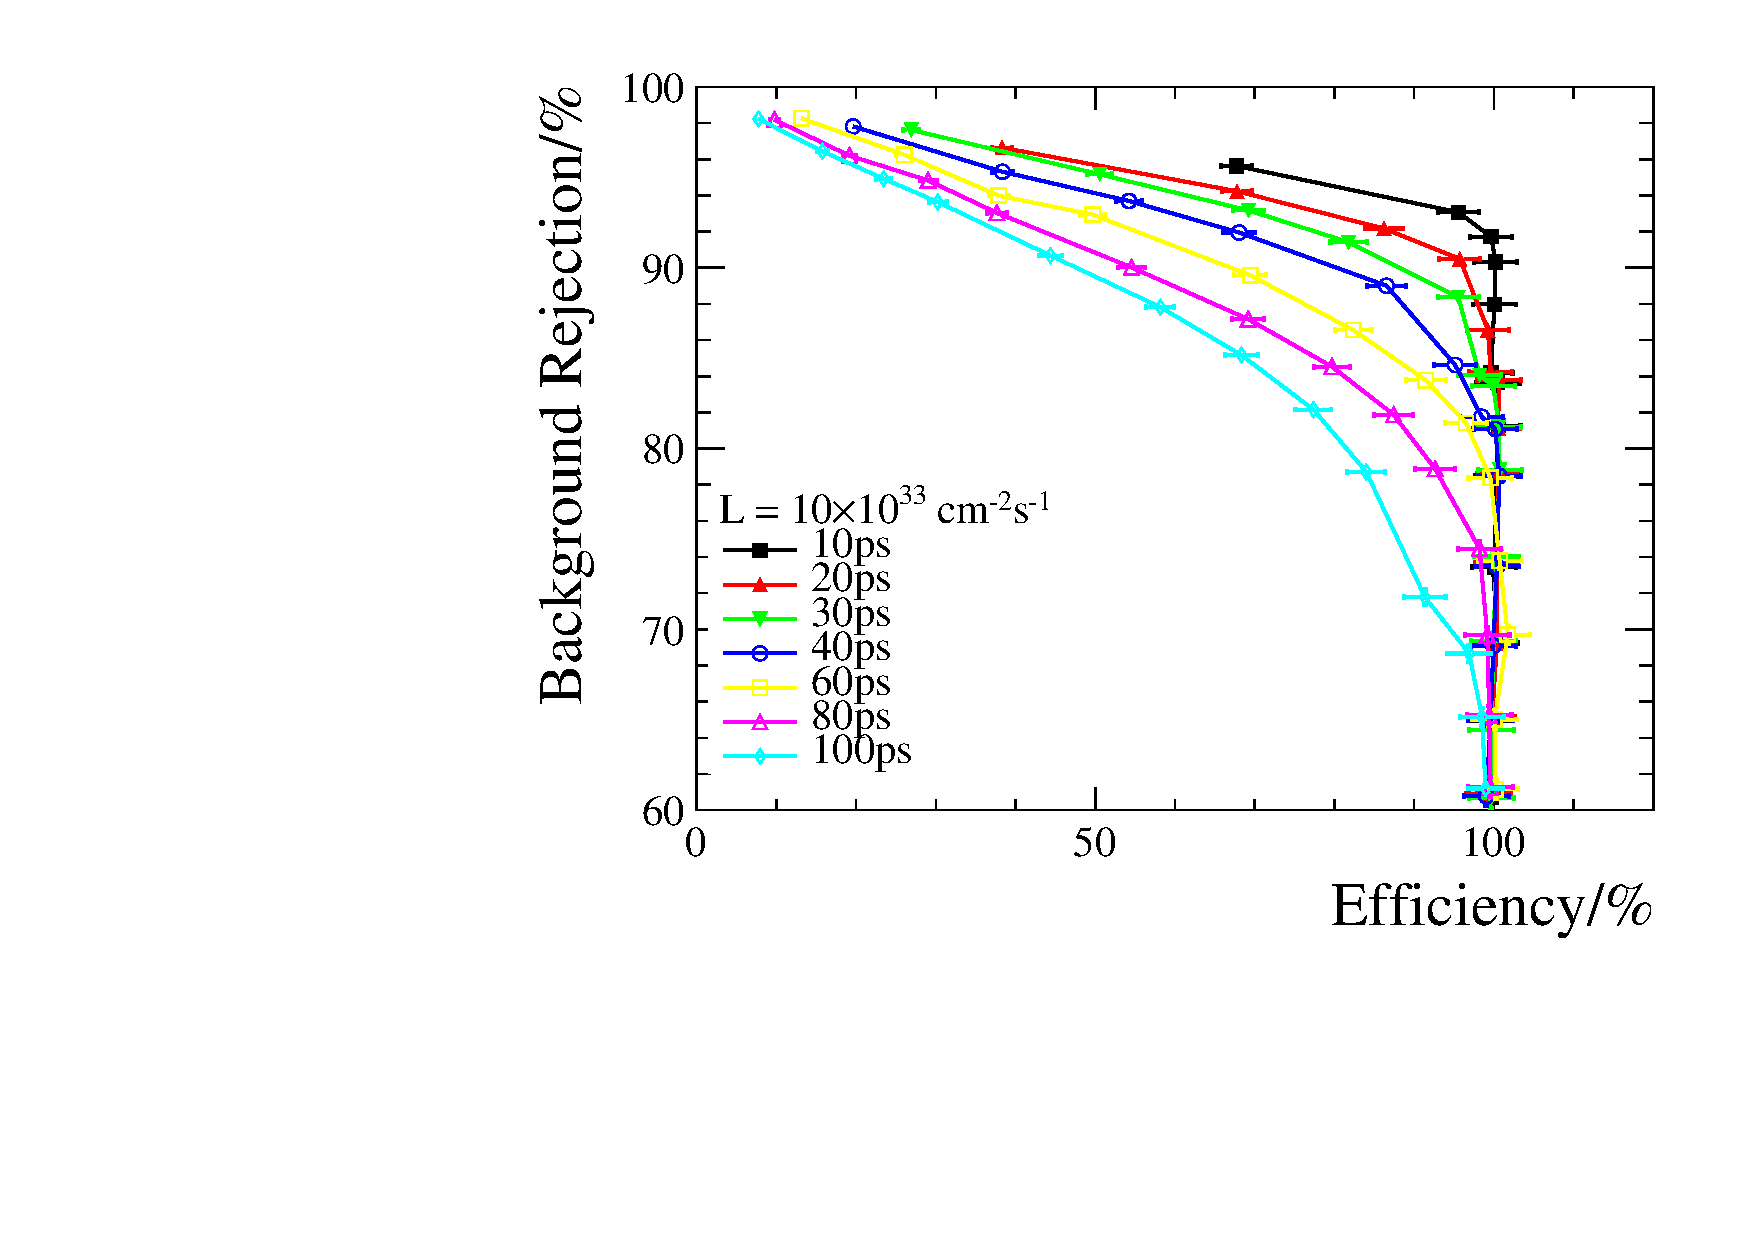
\includegraphics[width=0.45\linewidth]{Figures/06_ECAL/Fast_sim_Bs_PhiGamma/eff_vs_other/eff_vs_rej_Small_cell_Lumi_10_33_10.pdf} 
    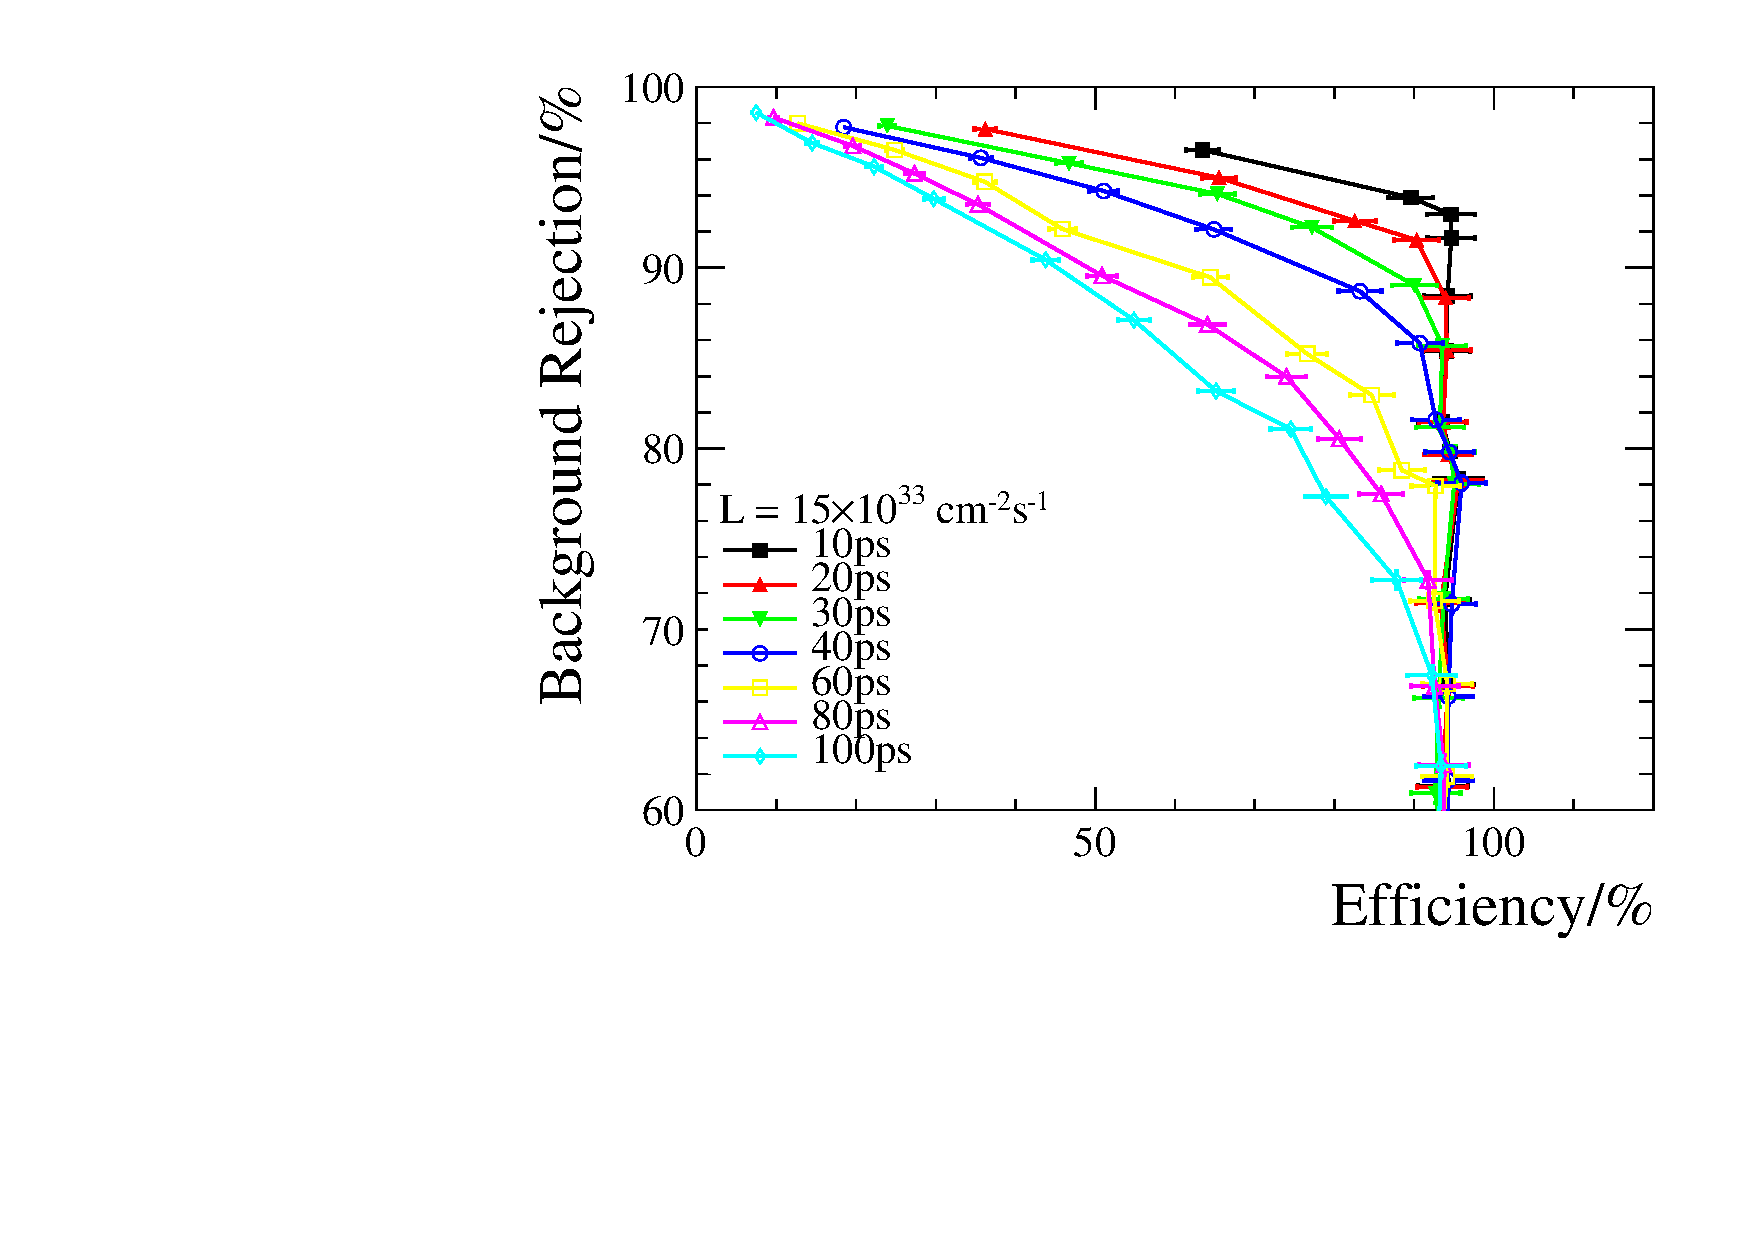
\includegraphics[width=0.45\linewidth]{Figures/06_ECAL/Fast_sim_Bs_PhiGamma/eff_vs_other/eff_vs_rej_Small_cell_Lumi_10_33_15.pdf}
    \\ 
    \vspace*{-0.5cm}
  \end{center}
  \caption{
  The relation between signal efficiency and combinatorial background rejection fraction with different $\Delta t$ cuts applied, 
   in Phillip's segmentation (top) and Si-W segmentation (bottom) respectively.
  }
  \label{fig:bs_phiGamma_phillip_eff_bkg}
\end{figure}
%%%%%%%%%%%%%%%%%%%%%%%%%%%%%%%%%%%%%%%%

The surge of combinatorial background comes from pile-up effect in high luminosity situation.
In order to remove this kind of background candidates,
the time information is used to distinguish the primary vertices.
Considering the \ecal can record the precision time information,
the shower time reconstructed from \ecal is named as $t_{1}$.
Assuming the futher \velo at \lhcb has ablity to detect the vertex time, 
named as $t_{2}$.
The time difference between the shower and vertex can be obtained as $\Delta t = t_{1}-t_{2}-l/c$, 
where $l/c$ represents the \g flight time.
In current simulation,
the time resolution of vertex is overlooked and the \ecal time resolution is given value.
In this way,
we can study the requirement of \ecal time resolution.

%%%%%%%%%%%%%%%%%%%%%%%%%%%%%%%%%%%%%%%%
\begin{figure}[!htb]
  \begin{center}
    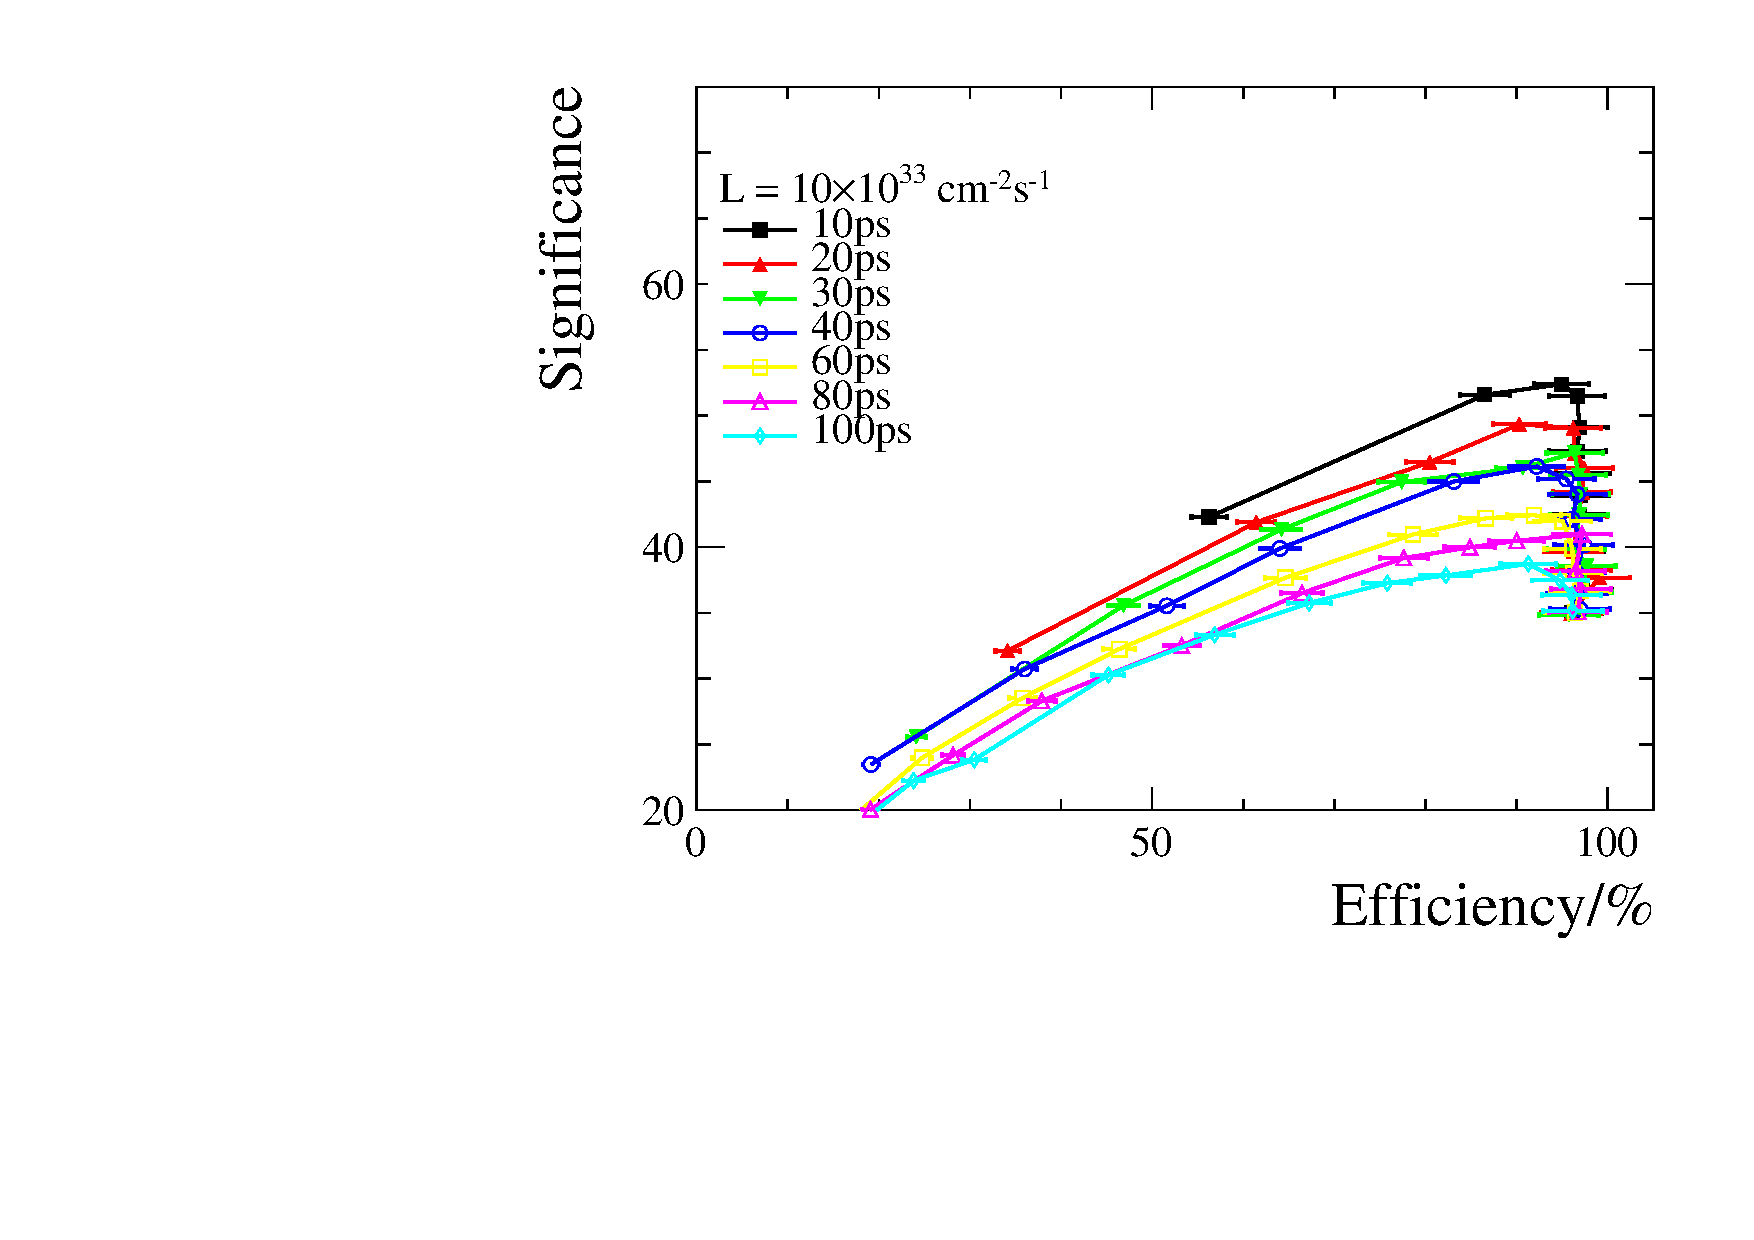
\includegraphics[width=0.45\linewidth]{Figures/06_ECAL/Fast_sim_Bs_PhiGamma/eff_vs_other/eff_vs_signi_Phillip_cell_Lumi_10_33_10.pdf} 
    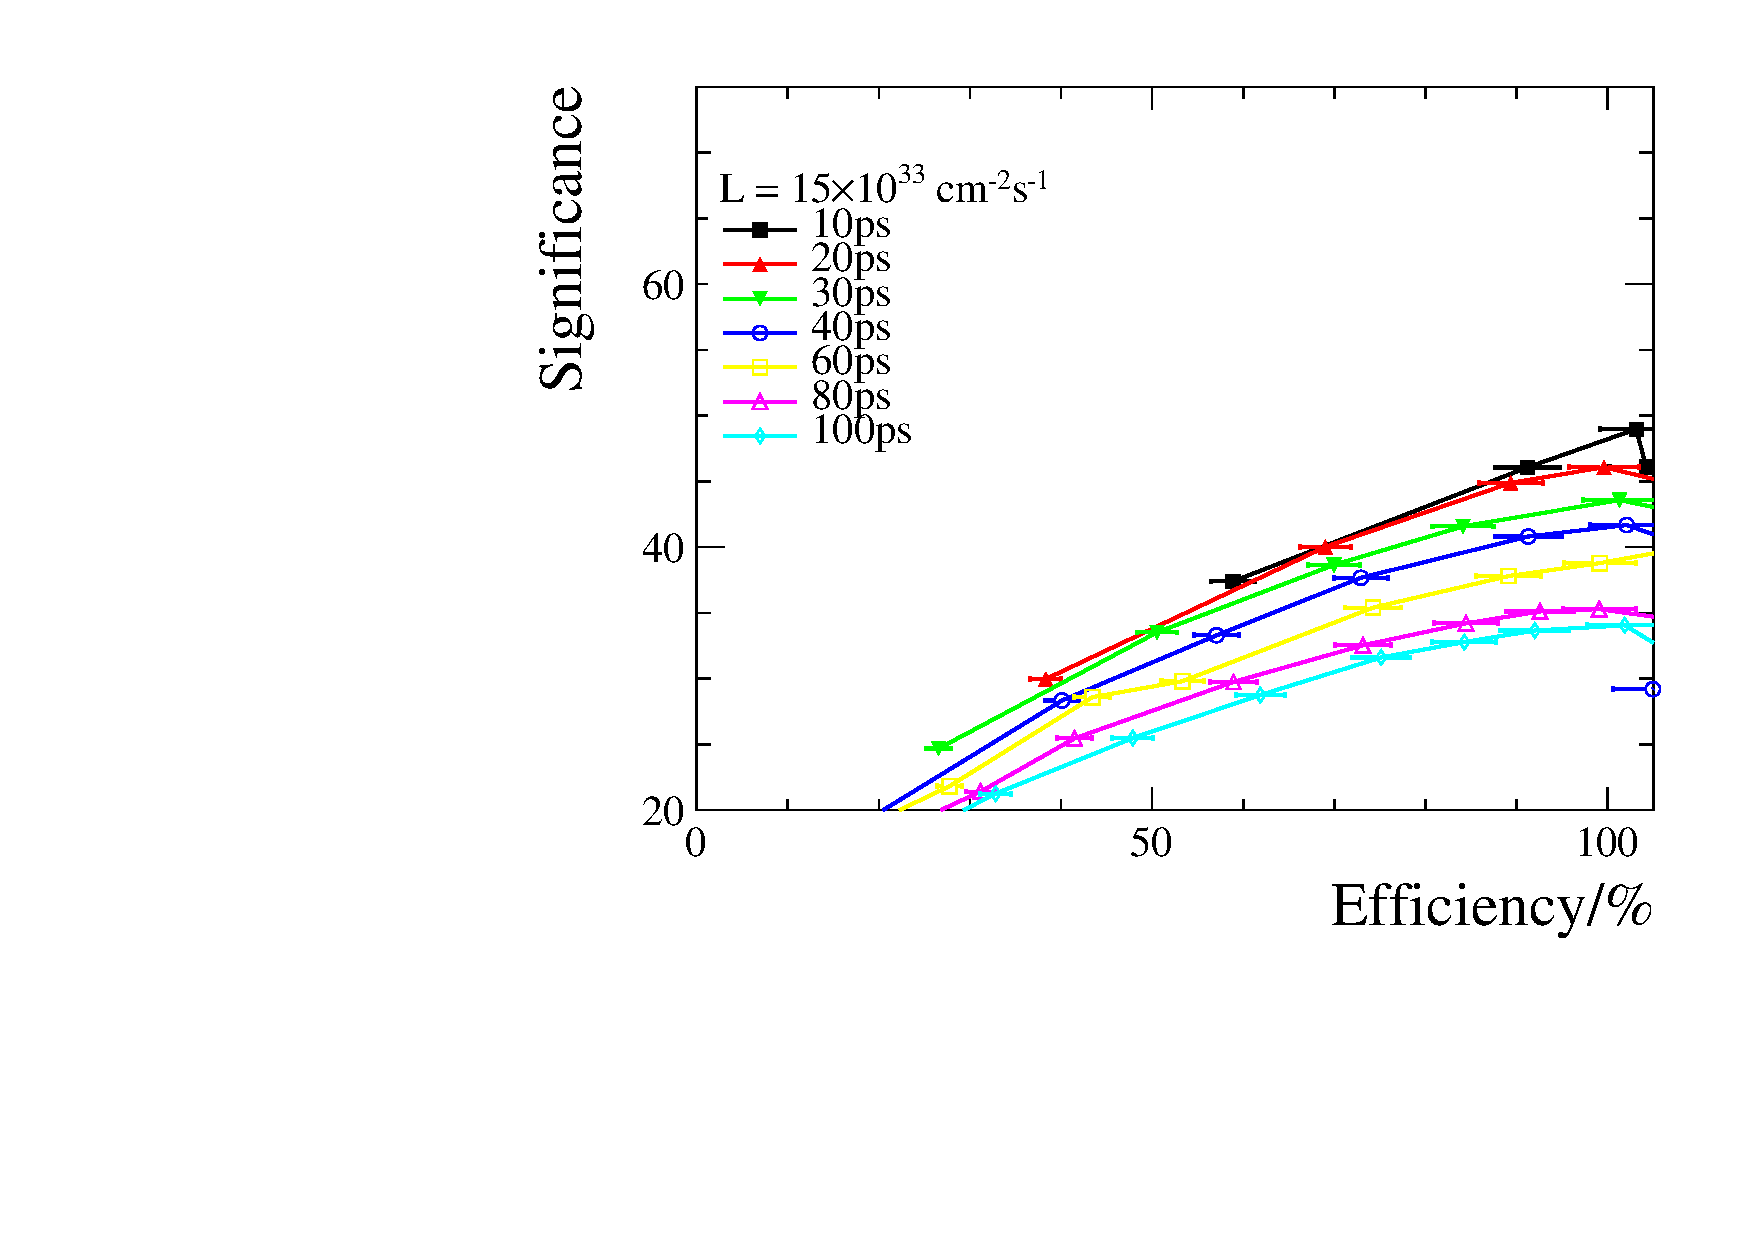
\includegraphics[width=0.45\linewidth]{Figures/06_ECAL/Fast_sim_Bs_PhiGamma/eff_vs_other/eff_vs_signi_Phillip_cell_Lumi_10_33_15.pdf}
    \\ 
    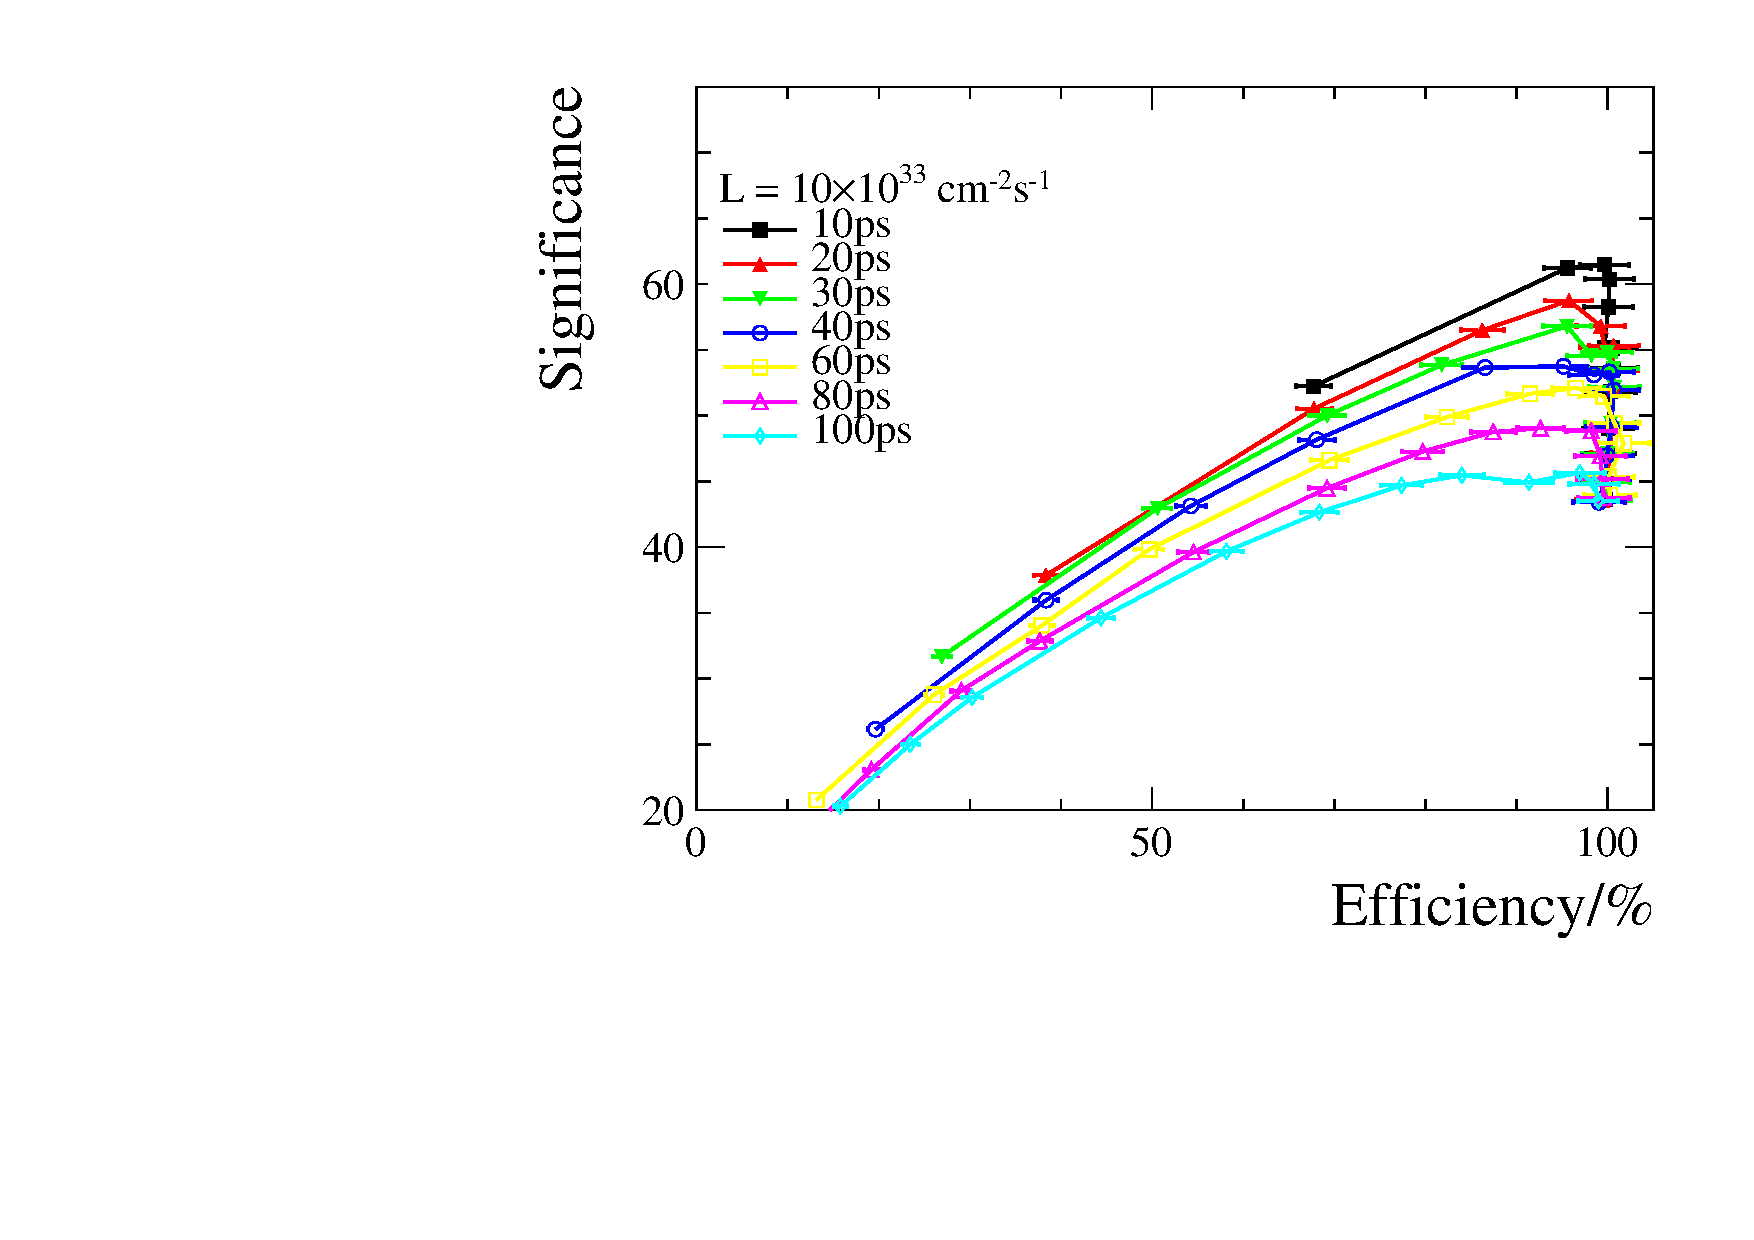
\includegraphics[width=0.45\linewidth]{Figures/06_ECAL/Fast_sim_Bs_PhiGamma/eff_vs_other/eff_vs_signi_Small_cell_Lumi_10_33_10.pdf} 
    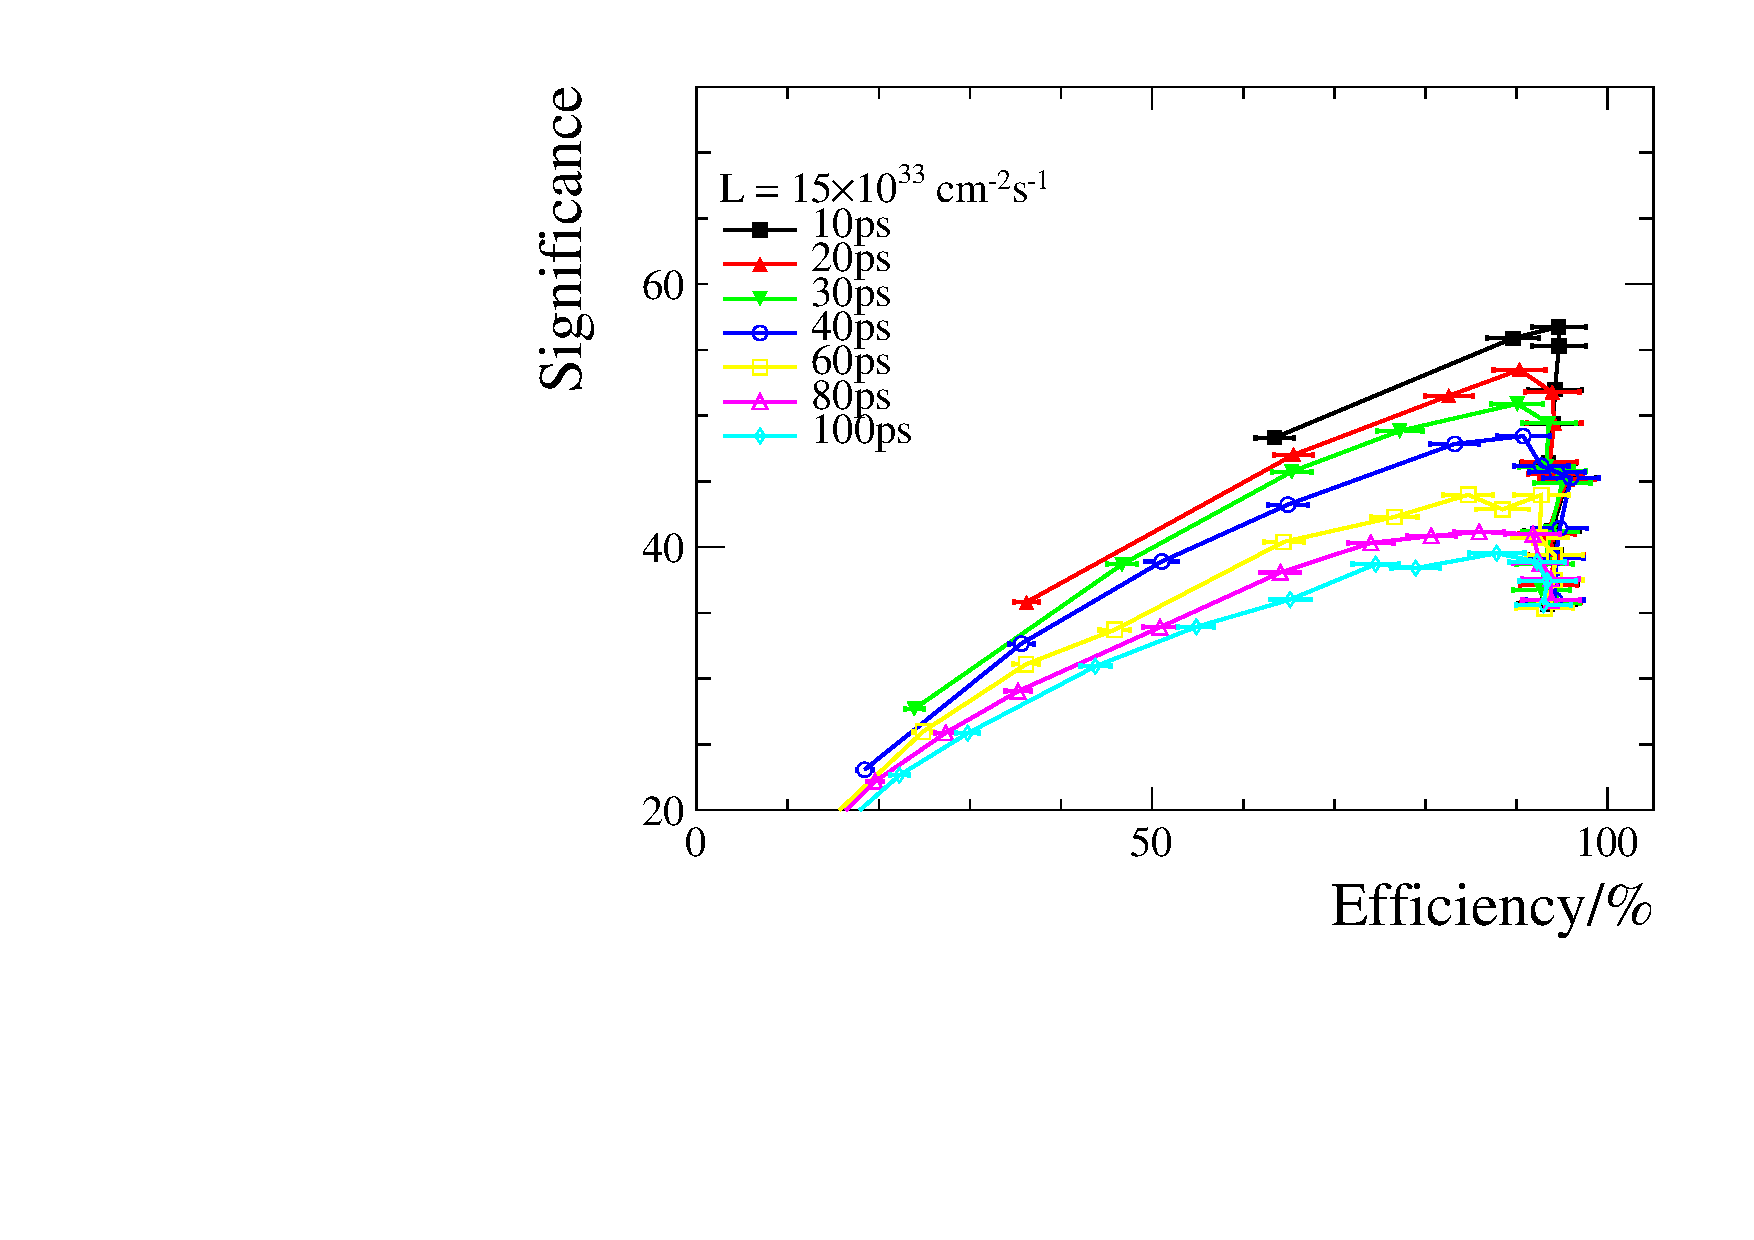
\includegraphics[width=0.45\linewidth]{Figures/06_ECAL/Fast_sim_Bs_PhiGamma/eff_vs_other/eff_vs_signi_Small_cell_Lumi_10_33_15.pdf}
    \\ 
    \vspace*{-0.5cm}
  \end{center}
  \caption{
  The relation between signal efficiency and significance with different $\Delta t$ cuts applied,
   in Phillip's segmentation (top) and Si-W segmentation (bottom) respectively.
  }
  \label{fig:bs_phiGamma_phillip_eff_sig}
\end{figure}
%%%%%%%%%%%%%%%%%%%%%%%%%%%%%%%%%%%%%%%%



The performances of this additional selection value $\Delta t$ in this decay channel is studied then.
The relation between selction efficiency and background rejection fraction after time matching applied with different time resolutions is shown in Figure.~\ref{fig:bs_phiGamma_phillip_eff_bkg}.
It is clearly that most of combinatorial background candidates can removed with the time resolution equal to tens of picosecond 
for both cell size segmentation.
The signel significance of $20000$ events simulation sample was also studied,
as shown in Figure.~\ref{fig:bs_phiGamma_phillip_eff_sig}.
Based on the research described above,
there is not a big challenge for this channel reconstruction in high luminosity situation,
tens of picosecond can help to reject most of combinatorial background candidates due to high pile-up effect.
Both Phillip's segmentation and Si-W segmentation have good performances.
Nevertheless,
we need to keep in mind mind that this channel can be studied during Run 1 and Run 2 at \lhcb,
the mentioned requirements to \ecal for this channel cannot expand study scope at \lhcb.  


\subsection{Performance in $\Bs\to\jpsi\piz$ decay}

Another interesing decay channel is $\Bs\to\jpsi\piz$,
which has not been observed yet.
Besides,
the channel $\Bd\to\jpsi\piz$ has similar topology to this one,
we can estimate the both channel together using same simulation samples for this pre-study.
The decay channel of $\Bs\to\jpsi\piz$ is studied with different \ecal cell size configration or luminosity condition. 
Similar to the $\Bs\to\phi\gamma$ decay study,
$\jpsi$ information is obtained from generated samples.
Table.~\ref{tab:ecal_bs2JpsiPiz} lists all selections used in this channel reconstruction,
the transverse energy of reconstructed gamma is larger than $0.5\gev$ and the transverse of the $\piz$ candidates greater than $2\gev$.
Besides,
the \piz candidates with mass in $2.5\sigma$ of \piz mass resolution are used to reconstruct \Bs.
In addition,
the transverse energy of \Bs is required to be larger than $2\gev$.

\begin{table}[tbh]
\caption{Selection criteria in $\Bs\to\jpsi\piz$ channel.}
\centering
\begin{tabular}{rl}
\hline
Quantity               	& Selections \\
\hline
\pt of \g           	& $>0.5 \gev$ \\
\pt of \piz           	& $>2 \gev$ \\
mass window of \piz 	& $2.5\sigma_{M}$ \\
\pt of \Bs			& $>2.0 \gev$ \\
\hline
\end{tabular}
\label{tab:ecal_bs2JpsiPiz}
\end{table}


\subsubsection{Luminosity effect}

The physical performances in this channel with different luminosities are studied first.
20000 simulation samples for each luminosities were generated by this parameterized simulation tool.
Figure.~\ref{fig:bs_Jpsipiz_diff_lumi} shows the $\jpsi\piz$ invariant mass distribution with different luminosities. 
The yields of signal and background are estimated by fitting the mass distribution for each smaple,
where the gaussian function is used to describe the shape of signal and the background is described 2 order chebyshev polynomial function.
The fitting results are listed in Table.~\ref{tab:ecal_bs2Jpsipiz_diff_lumi}.
This channel is different from $\Bs\to\phi\g$,
the number of background candidates grows even faster as luminosity increases,
aspecially in the $\lum=1.5\times10^{34}\cm^{-2}\cdot\sec^{-1}$ case.
The reason is that two \g candidates are used in reconstruction for this channel,
and everage energy of \g in this channel is usually smaller than the value in $\Bs\to\phi\g$ decay.
By the way,
the significance is defined as $S/\sqrt{S+20\dot B}$ here.
The backgound yield is multiplied with a factor of 20
\footnote{The factor of 20 is obtained from internal $\Bd\to\jpsi\piz$ analysis at \lhcb. } 
as this value is underestimated from signal simulation sample.

%%%%%%%%%%%%%%%%%%%%%%%%%%%%%%%%%%%%%%%%
\begin{figure}[!htb]
  \begin{center}
    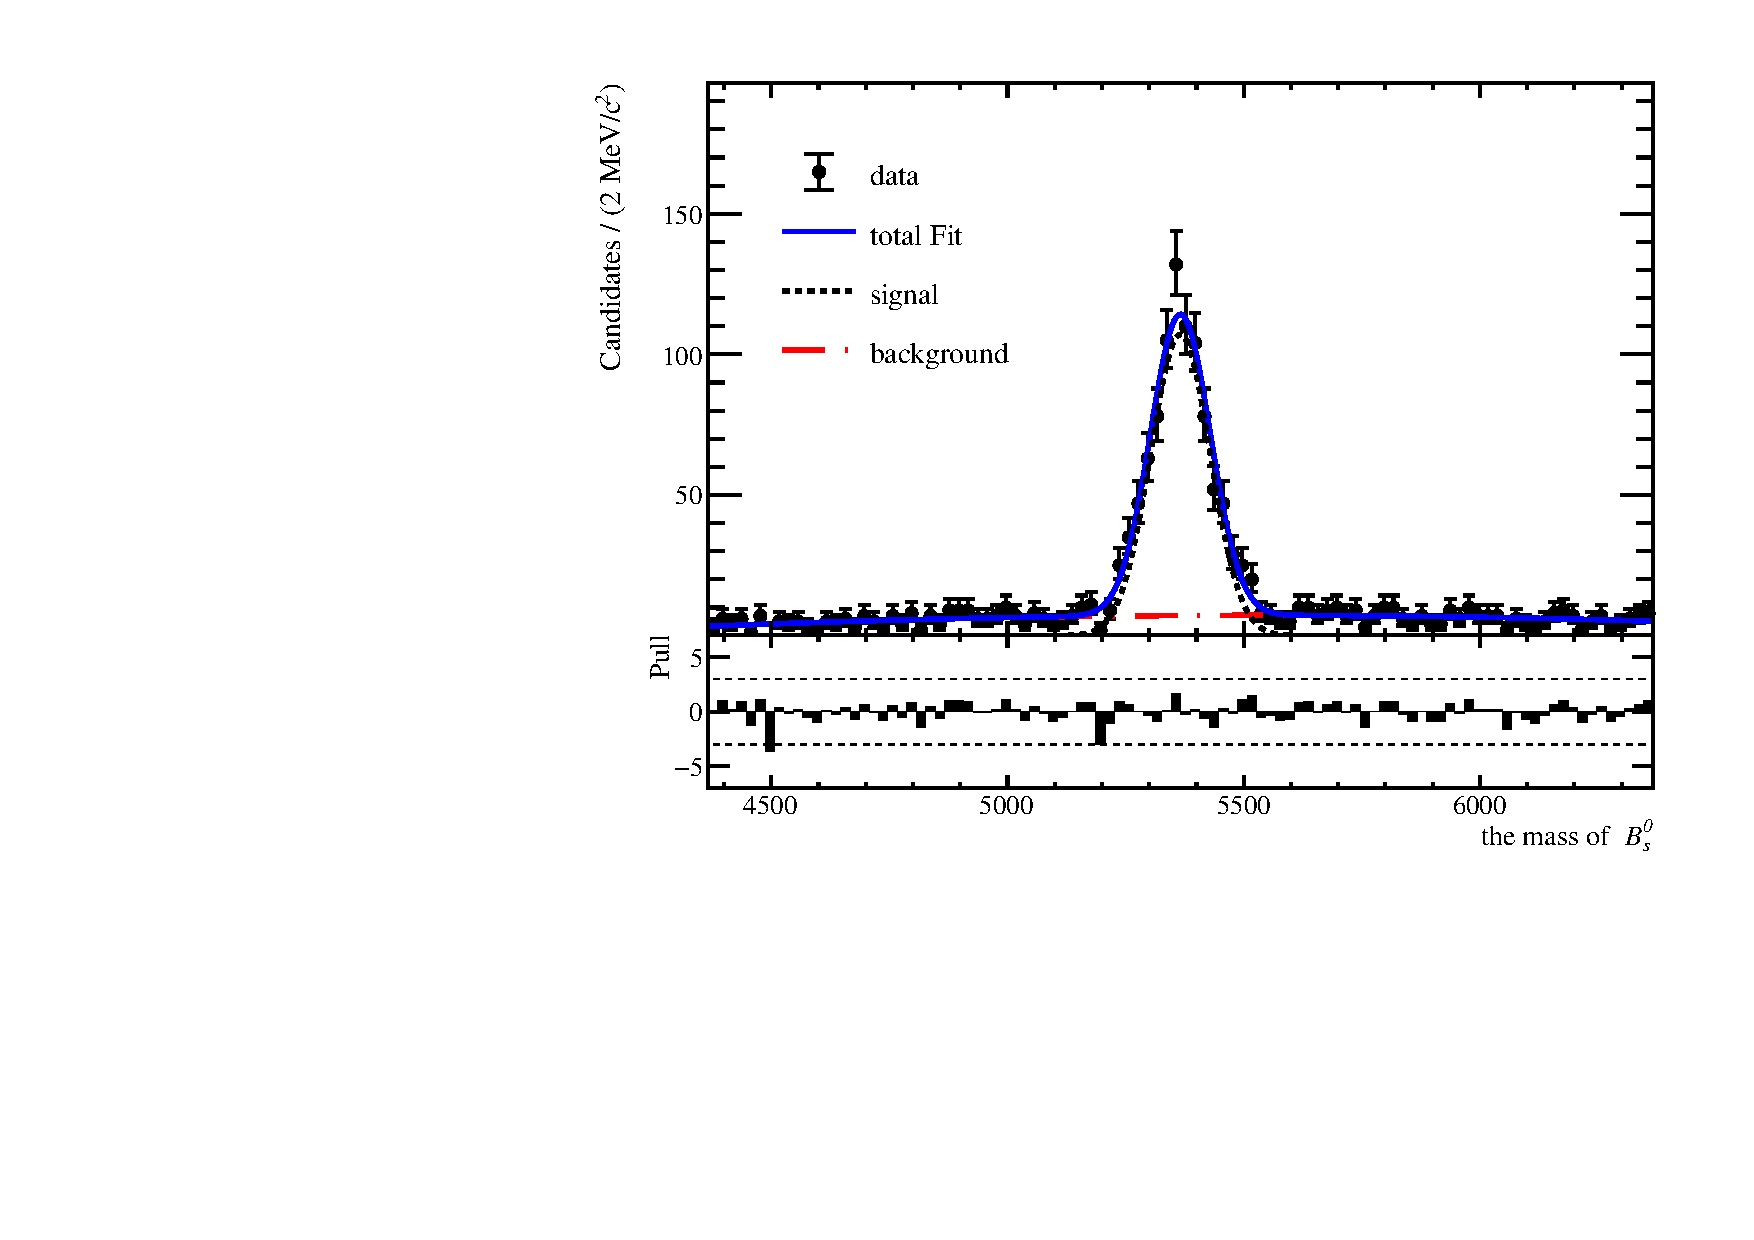
\includegraphics[width=0.45\linewidth]{Figures/06_ECAL/Fast_sim_Bs_JpsiPiz/bs0_pdf/Big_cell/Lumi_10_32_4/plot0.pdf}
    \put(-130,146) {\textrm{\small $\lum=4\times10^{32}\cm^{-2}\cdot\sec^{-1}$}}
    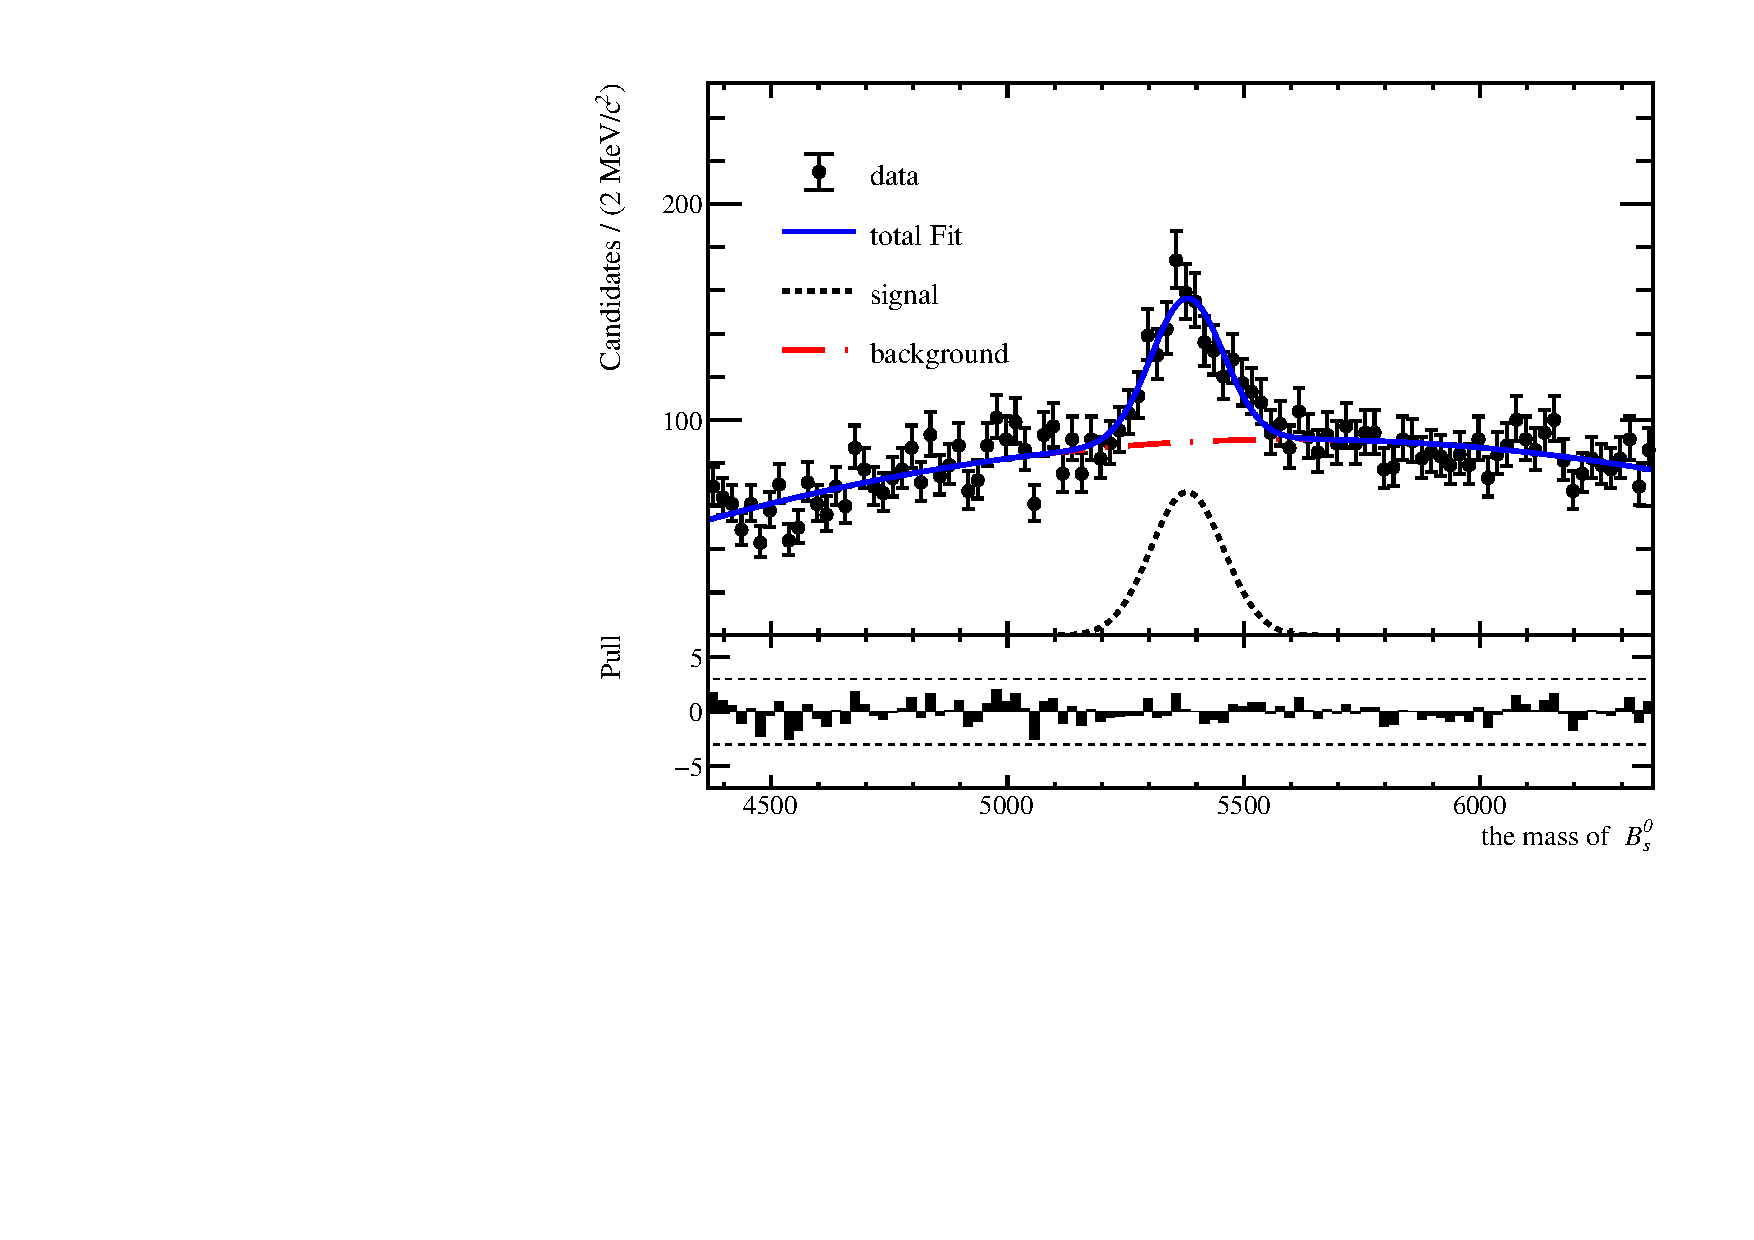
\includegraphics[width=0.45\linewidth]{Figures/06_ECAL/Fast_sim_Bs_JpsiPiz/bs0_pdf/Big_cell/Lumi_10_33_6/plot0.pdf}
    \put(-130,146) {\textrm{\small $\lum=0.6\times10^{34}\cm^{-2}\cdot\sec^{-1}$}}
    \\ 
    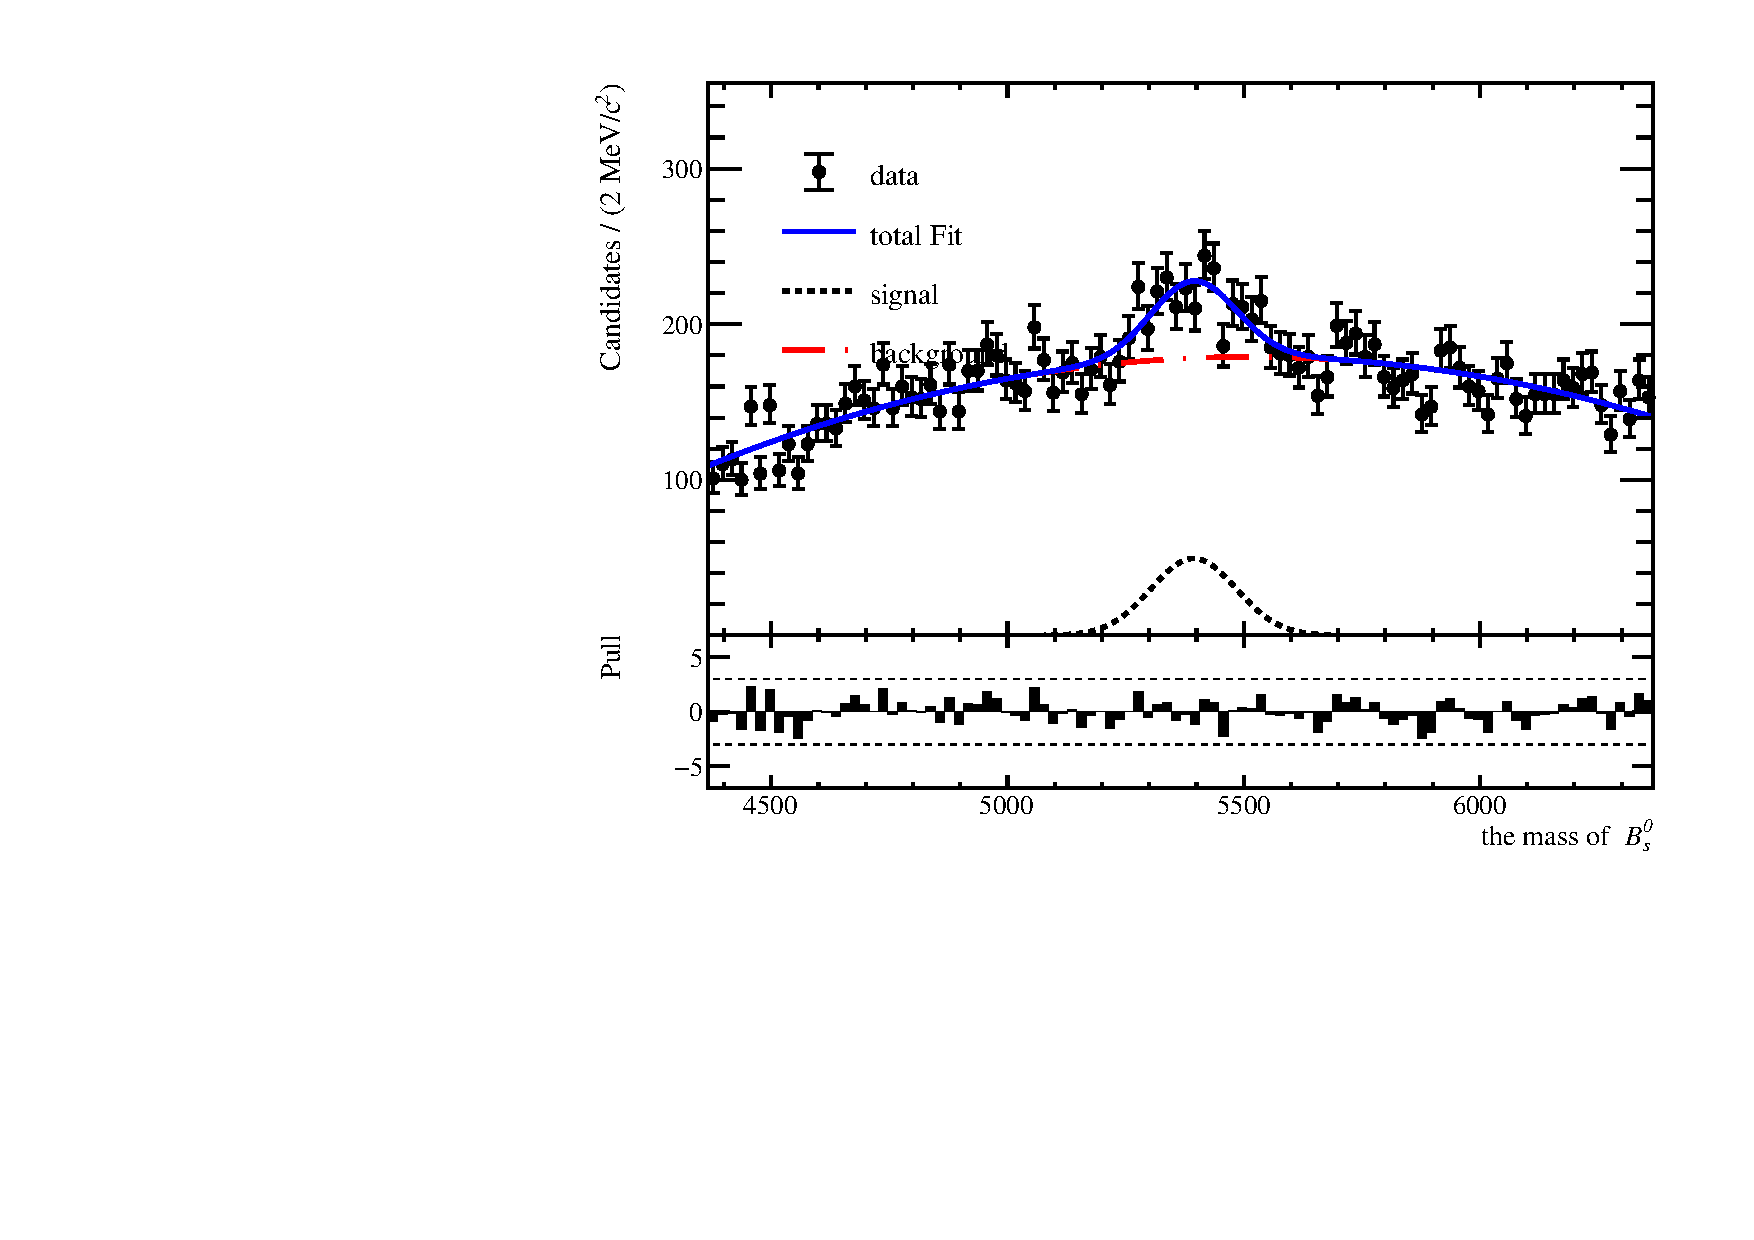
\includegraphics[width=0.45\linewidth]{Figures/06_ECAL/Fast_sim_Bs_JpsiPiz/bs0_pdf/Big_cell/Lumi_10_33_10/plot0.pdf} 
    \put(-130,146) {\textrm{\small $\lum=1.0\times10^{34}\cm^{-2}\cdot\sec^{-1}$}}
    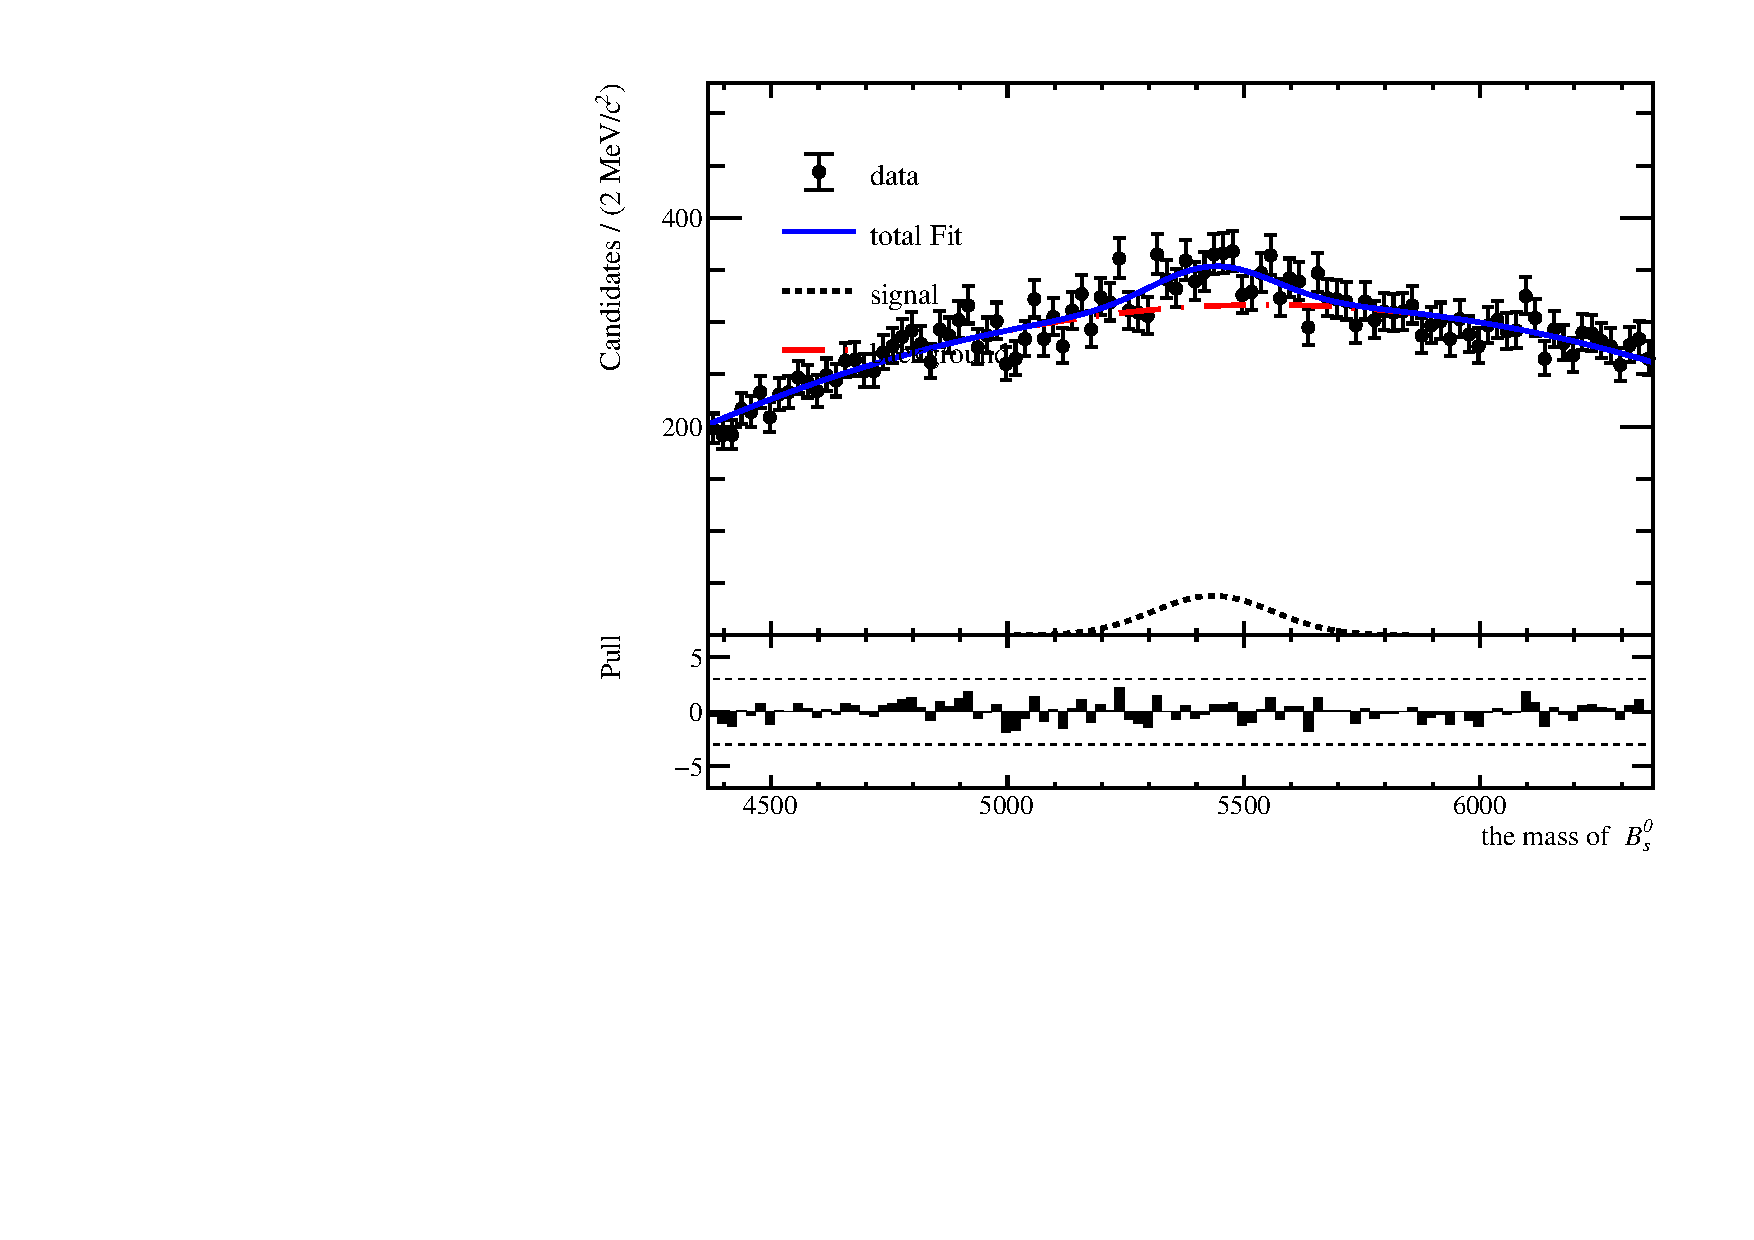
\includegraphics[width=0.45\linewidth]{Figures/06_ECAL/Fast_sim_Bs_JpsiPiz/bs0_pdf/Big_cell/Lumi_10_33_15/plot0.pdf}
    \put(-130,146) {\textrm{\small $\lum=1.5\times10^{34}\cm^{-2}\cdot\sec^{-1}$}}
    \\ 
    \vspace*{-0.5cm}
  \end{center}
  \caption{
     The mass distribution of $\Bs$ in $\Bs\to\jpsi\piz$ decay with different luminosities.
  }
  \label{fig:bs_Jpsipiz_diff_lumi}
\end{figure}
%%%%%%%%%%%%%%%%%%%%%%%%%%%%%%%%%%%%%%%%


\subsubsection{Smaller cell size to improve the reconstruction efficiency}

\begin{table}[!tbh]
\caption{The physical performance in different luminosities with different \ecal cell segmentation.}
\centering
\begin{tabular}{ c | c c c c c}
\hline\hline
   Segmentation 
   & \tabincell{c}{Luminosity \\ ($\cm^{-2}\cdot\sec^{-1}$) } 
   %& \tabincell{c}{(-19.37,\\+9.53  )}
   & Efficiency	
   & \tabincell{c}{Bkg \\ ($\times1000$)	}	
   & Significance	
   & \tabincell{c}{Mass resolution \\ (\mev) } \\
\hline
\multirow{4}{*}{Current} &
$4\times10^{32}$           		& $0.042$		& $0.6$	     & $15$		    & $63$ \\
\cline{2-6} &
$0.6\times10^{34}$			& $0.032$ 		& $8.1$         & $3$            & $77$ \\
\cline{2-6} &
$1.0\times10^{34}$			& $0.028$ 		& $16.0$         & $2$            & $90$ \\
\cline{2-6} &
$1.5\times10^{34}$			& $-$ 		& $-$            & $-$            & $-$ \\
\hline
\multirow{4}{*}{Phillip's} &
$4\times10^{32}$           		& $0.071$		& $0.7$	     & $21$		     & $65$ \\
\cline{2-6} &
$0.6\times10^{34}$			& $0.059$ 		& $7.5$          & $7$            & $68$ \\
\cline{2-6} &
$1.0\times10^{34}$			& $0.059$ 		& $13.0$         & $5$            & $70$ \\
\cline{2-6} &
$1.5\times10^{34}$			& $0.039$ 		& $21.7$         & $3$            & $64$ \\
\hline
\multirow{4}{*}{Si-W} &
$4\times10^{32}$           		& $0.168$		& $1.3$		& $34$		& $82$ \\
\cline{2-6} &
$0.6\times10^{34}$			& $0.153$ 		& $12.4$         & $13$            & $77$ \\
\cline{2-6} &
$1.0\times10^{34}$			& $0.147$ 		& $21.1$         & $9$            & $79$ \\
\cline{2-6} &
$1.5\times10^{34}$			& $0.137$ 		& $33.7$         & $7$            & $77$ \\
\hline
\hline
\end{tabular}
\label{tab:ecal_bs2Jpsipiz_diff_lumi}
\end{table}

Similar to the study of $\Bs\to\phi\gamma$ decay,
all results with different simulation configurations are summaried in Table.~\ref{tab:ecal_bs2Jpsipiz_diff_lumi}.
According to these simulation samples,
we find that the reconstruction efficiencies change significantly,
which is much different from the decay of $\Bs\to\phi\gamma$.
The signal reconstruction efficiency of Si-W small cell size segmentation is around 4 times larger than the number of current \ecal segmentation.
Besides, 
the number of background candidates are pretty large in high luminosity situation for each case.
There is not chance to study this channel if the combinatorial background candidates cannot be rejected.


\subsubsection{Precision timing to remove pile-up effect}

%%%%%%%%%%%%%%%%%%%%%%%%%%%%%%%%%%%%%%%%
\begin{figure}[!htb]
  \begin{center}
    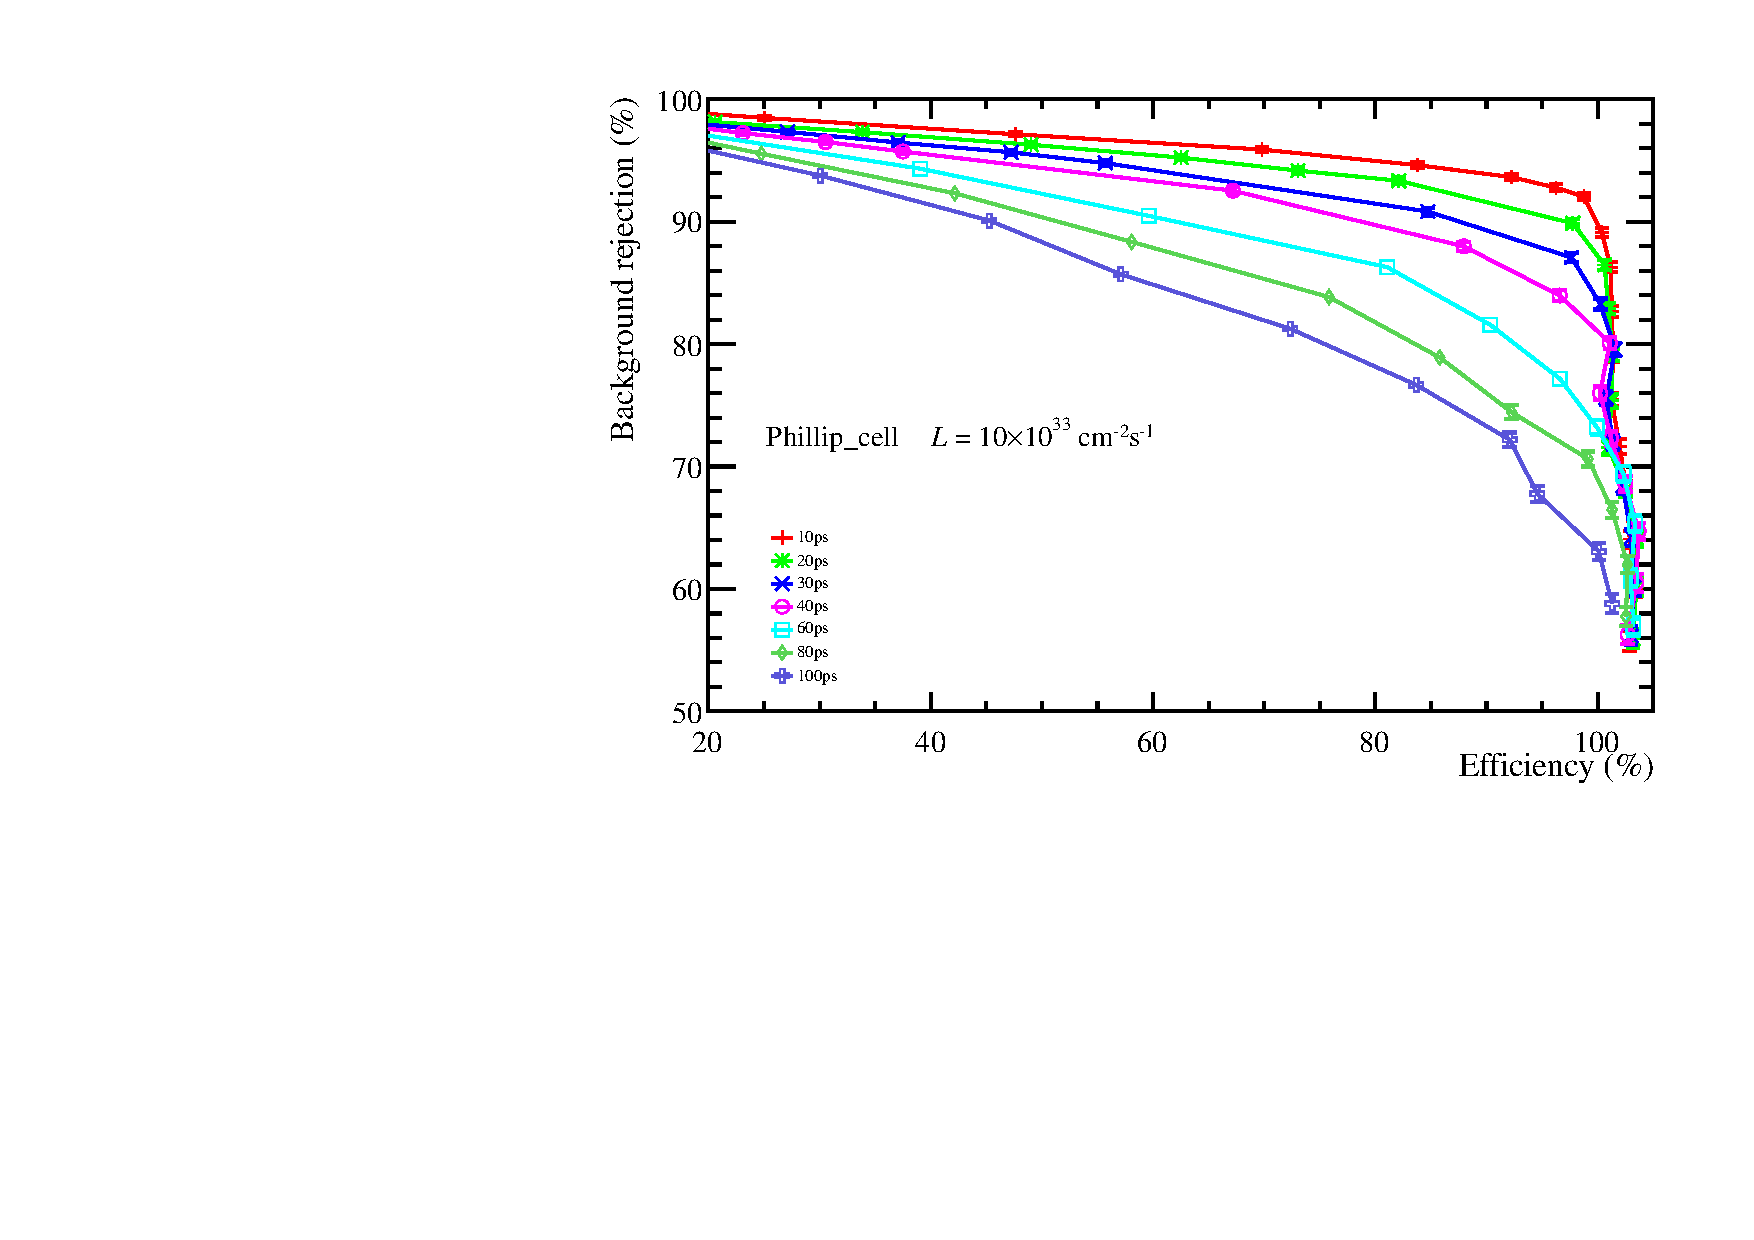
\includegraphics[width=0.45\linewidth]{Figures/06_ECAL/Fast_sim_Bs_JpsiPiz/eff_sig/Phillip_cell_Lumi_10_33_10_eff_bkg.pdf} 
    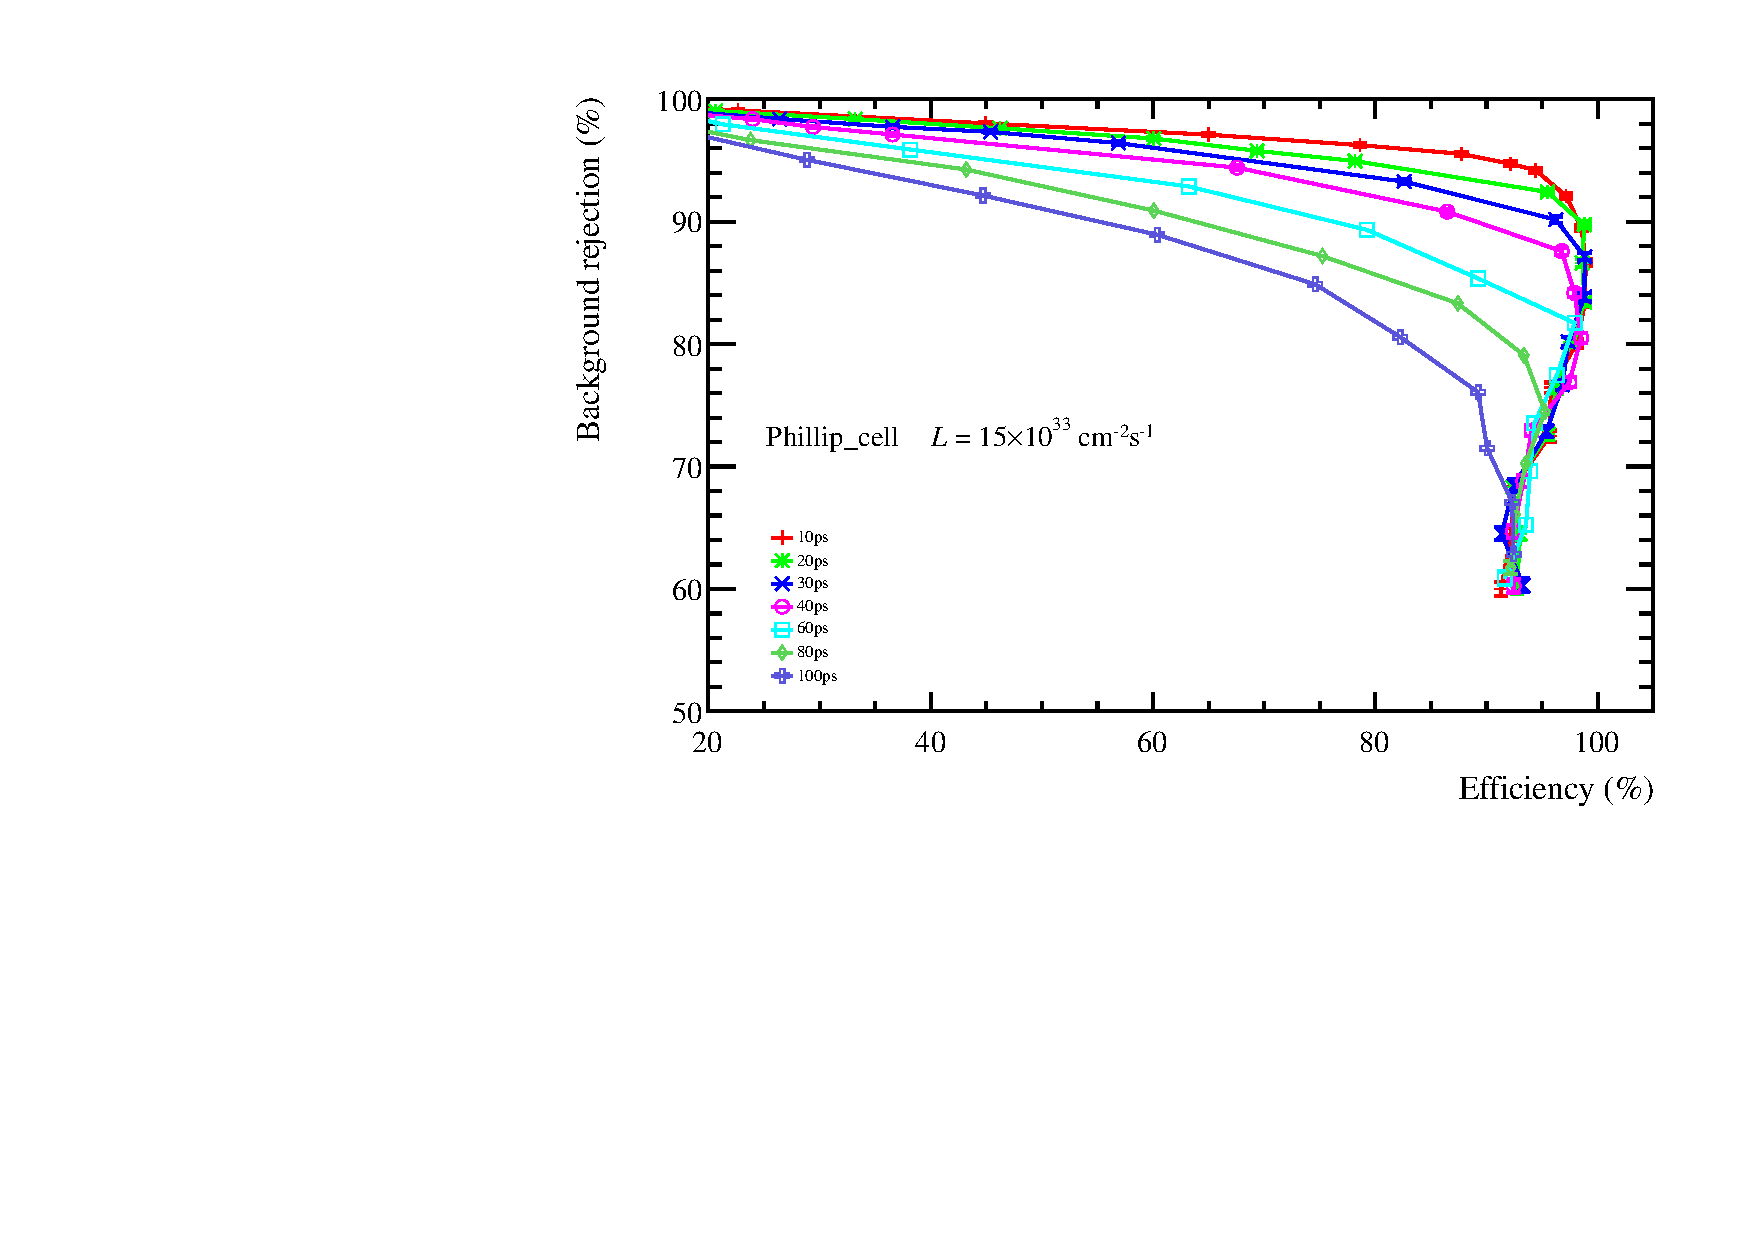
\includegraphics[width=0.45\linewidth]{Figures/06_ECAL/Fast_sim_Bs_JpsiPiz/eff_sig/Phillip_cell_Lumi_10_33_15_eff_bkg.pdf}
    \\ 
    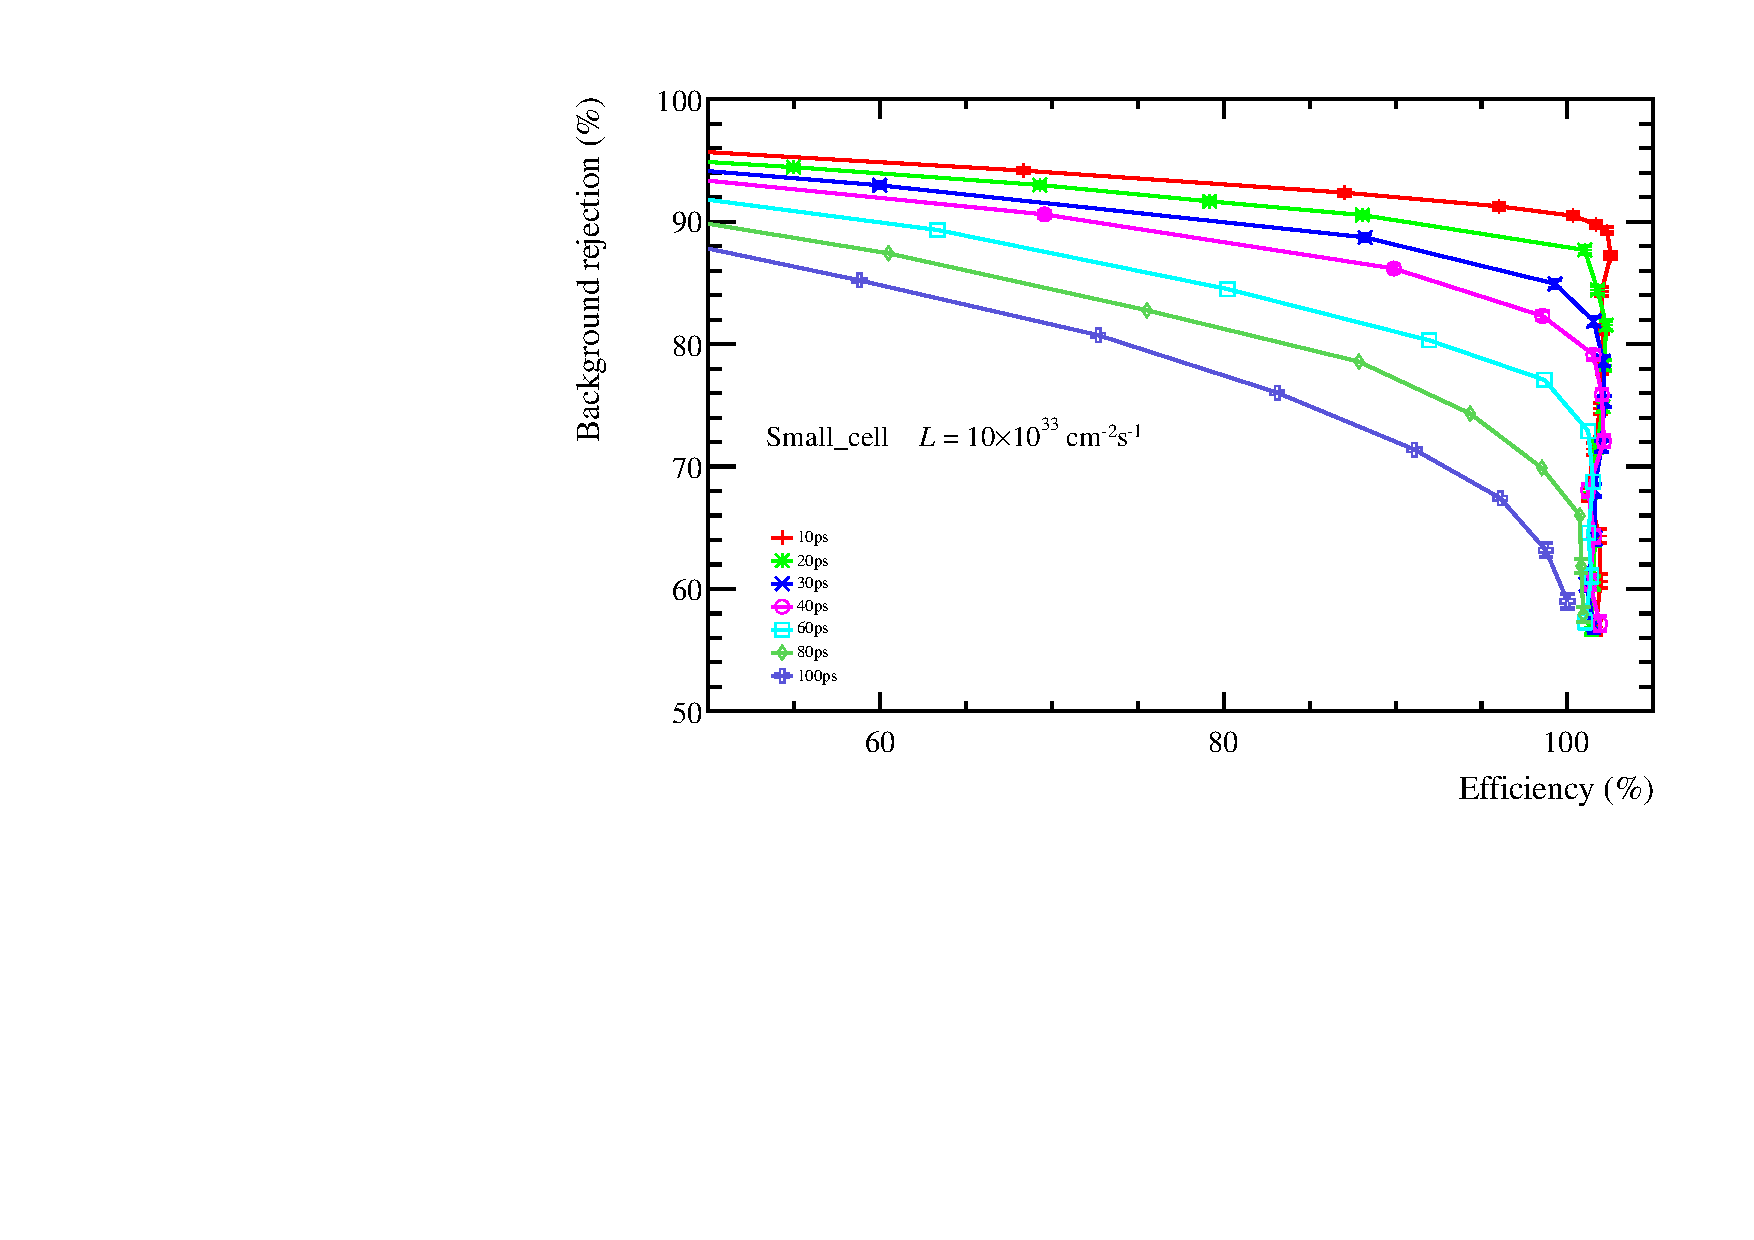
\includegraphics[width=0.45\linewidth]{Figures/06_ECAL/Fast_sim_Bs_JpsiPiz/eff_sig/Small_cell_Lumi_10_33_10_eff_bkg.pdf} 
    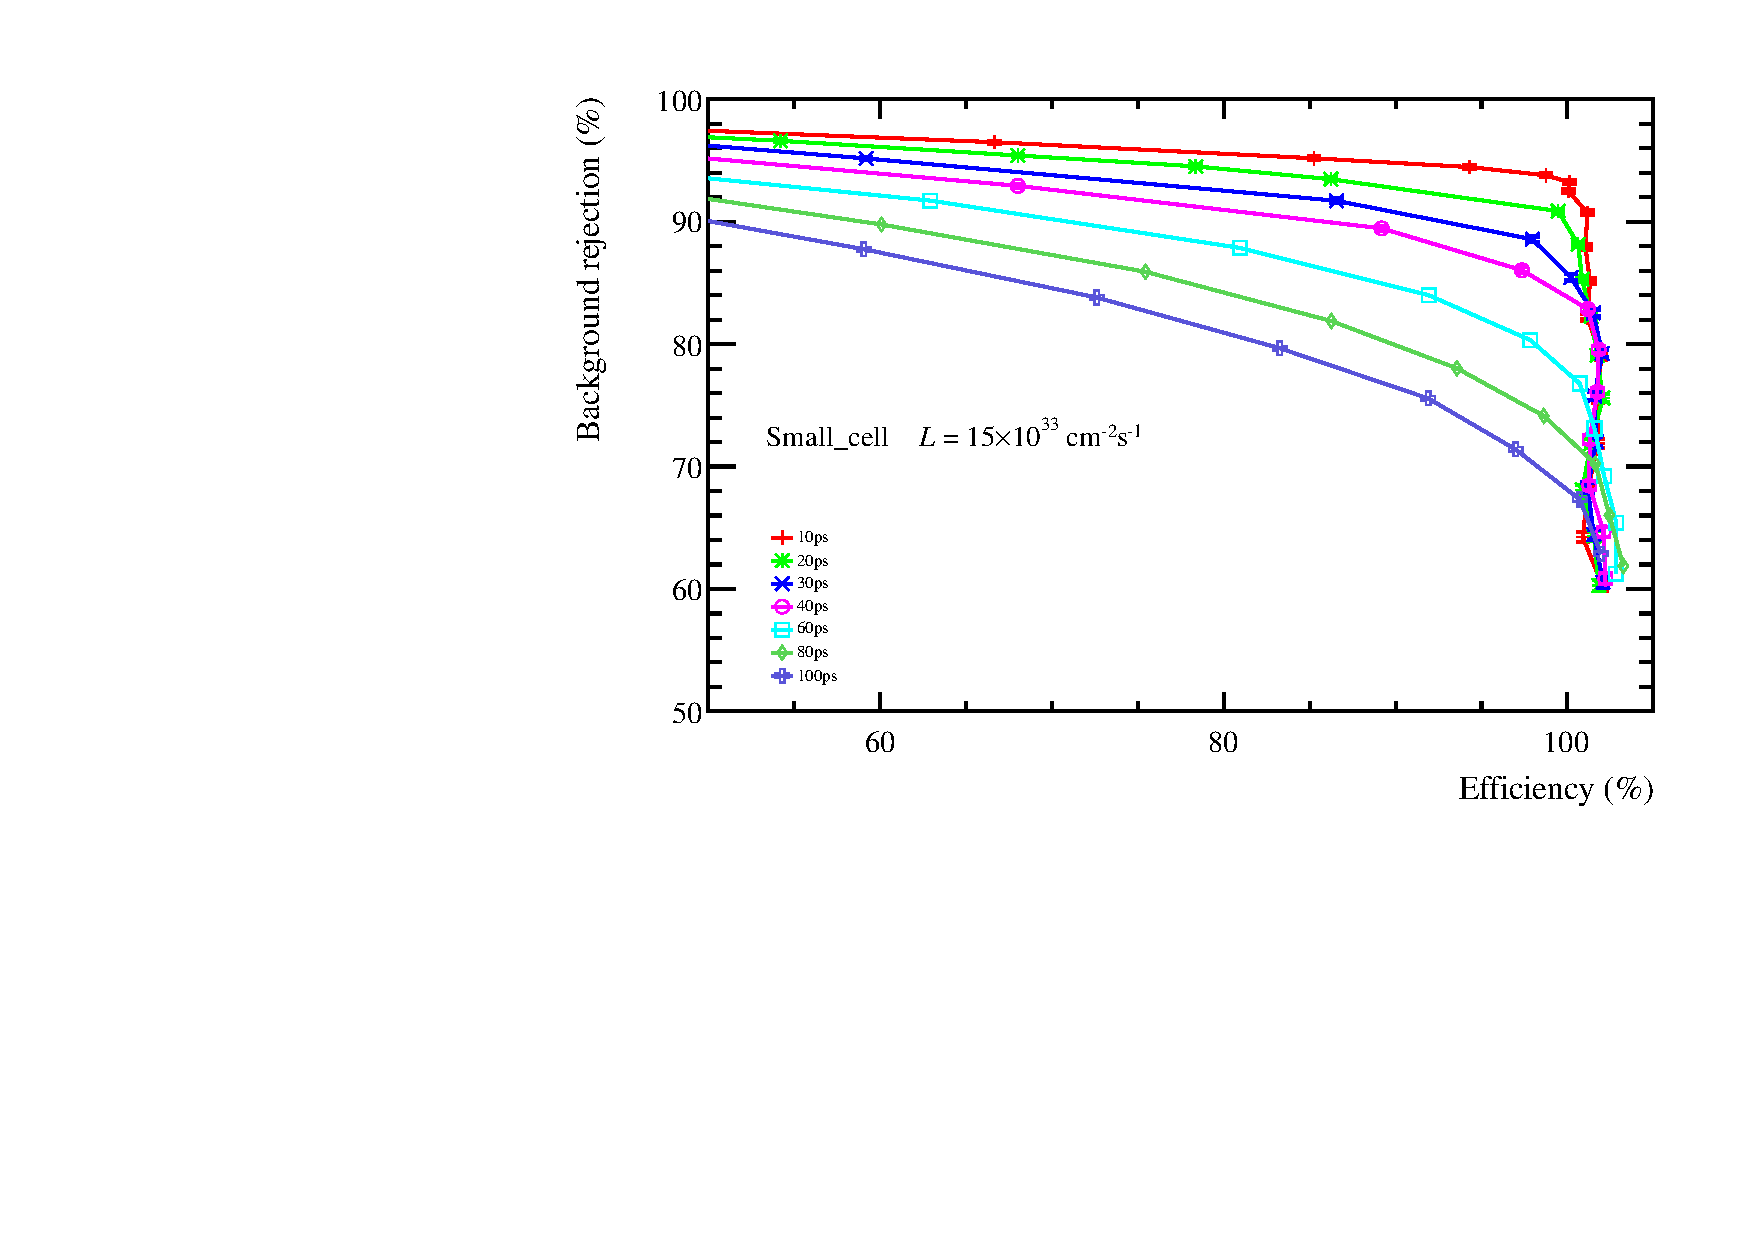
\includegraphics[width=0.45\linewidth]{Figures/06_ECAL/Fast_sim_Bs_JpsiPiz/eff_sig/Small_cell_Lumi_10_33_15_eff_bkg.pdf}
    \\ 
    \vspace*{-0.5cm}
  \end{center}
  \caption{
     The relation between signal efficiency and combinatorial background rejection fraction with different $R(t)$ cuts applied, 
   in Phillip's segmentation (top) and Si-W segmentation (bottom) respectively.
  }
  \label{fig:bs_Jpsipiz_phillip_eff_bkg}
\end{figure}
%%%%%%%%%%%%%%%%%%%%%%%%%%%%%%%%%%%%%%%%

High luminosity leads to a pretty high combinatorial background level. 
In order to remove this kind of background candidates,
the time information is used to distinguish the primary vertices.
Unlike the $\Bs\to\phi\gamma$,
two \g are used in this channel reconstruction.
A new variable $R(t)$ is used to reject background candidates, 
which is defined as $R(t)=\sqrt{\Delta(t_{1})^2 + \Delta(t_{2})^2}$,
where the $\Delta(t_{1})$ is the difference between the \jpsi vertex time and expected \g generated time measured by \ecal, 
$\Delta(t_{2})$ the denotes the time difference of the other \g.

%%%%%%%%%%%%%%%%%%%%%%%%%%%%%%%%%%%%%%%%
\begin{figure}[!htb]
  \begin{center}
    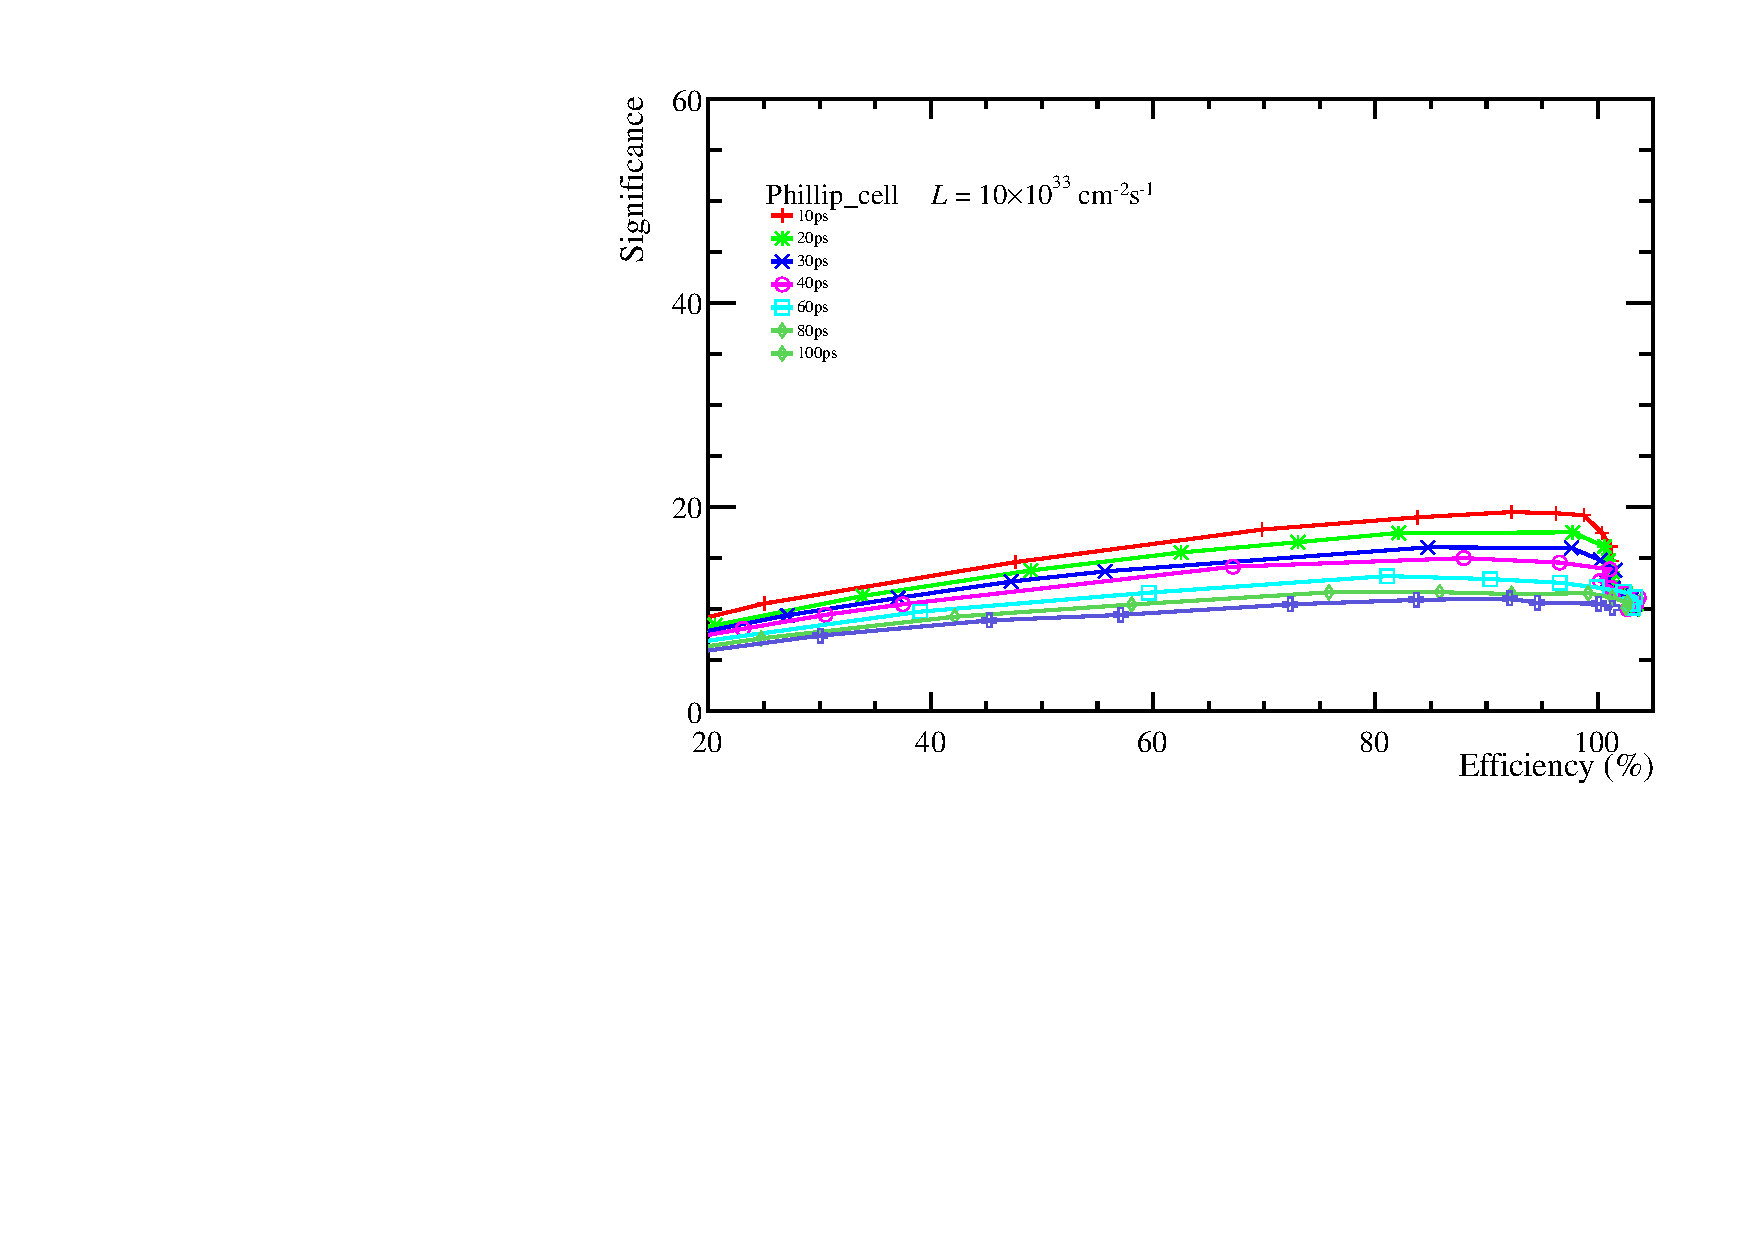
\includegraphics[width=0.45\linewidth]{Figures/06_ECAL/Fast_sim_Bs_JpsiPiz/eff_sig/Phillip_cell_Lumi_10_33_10_eff_signi.pdf} 
    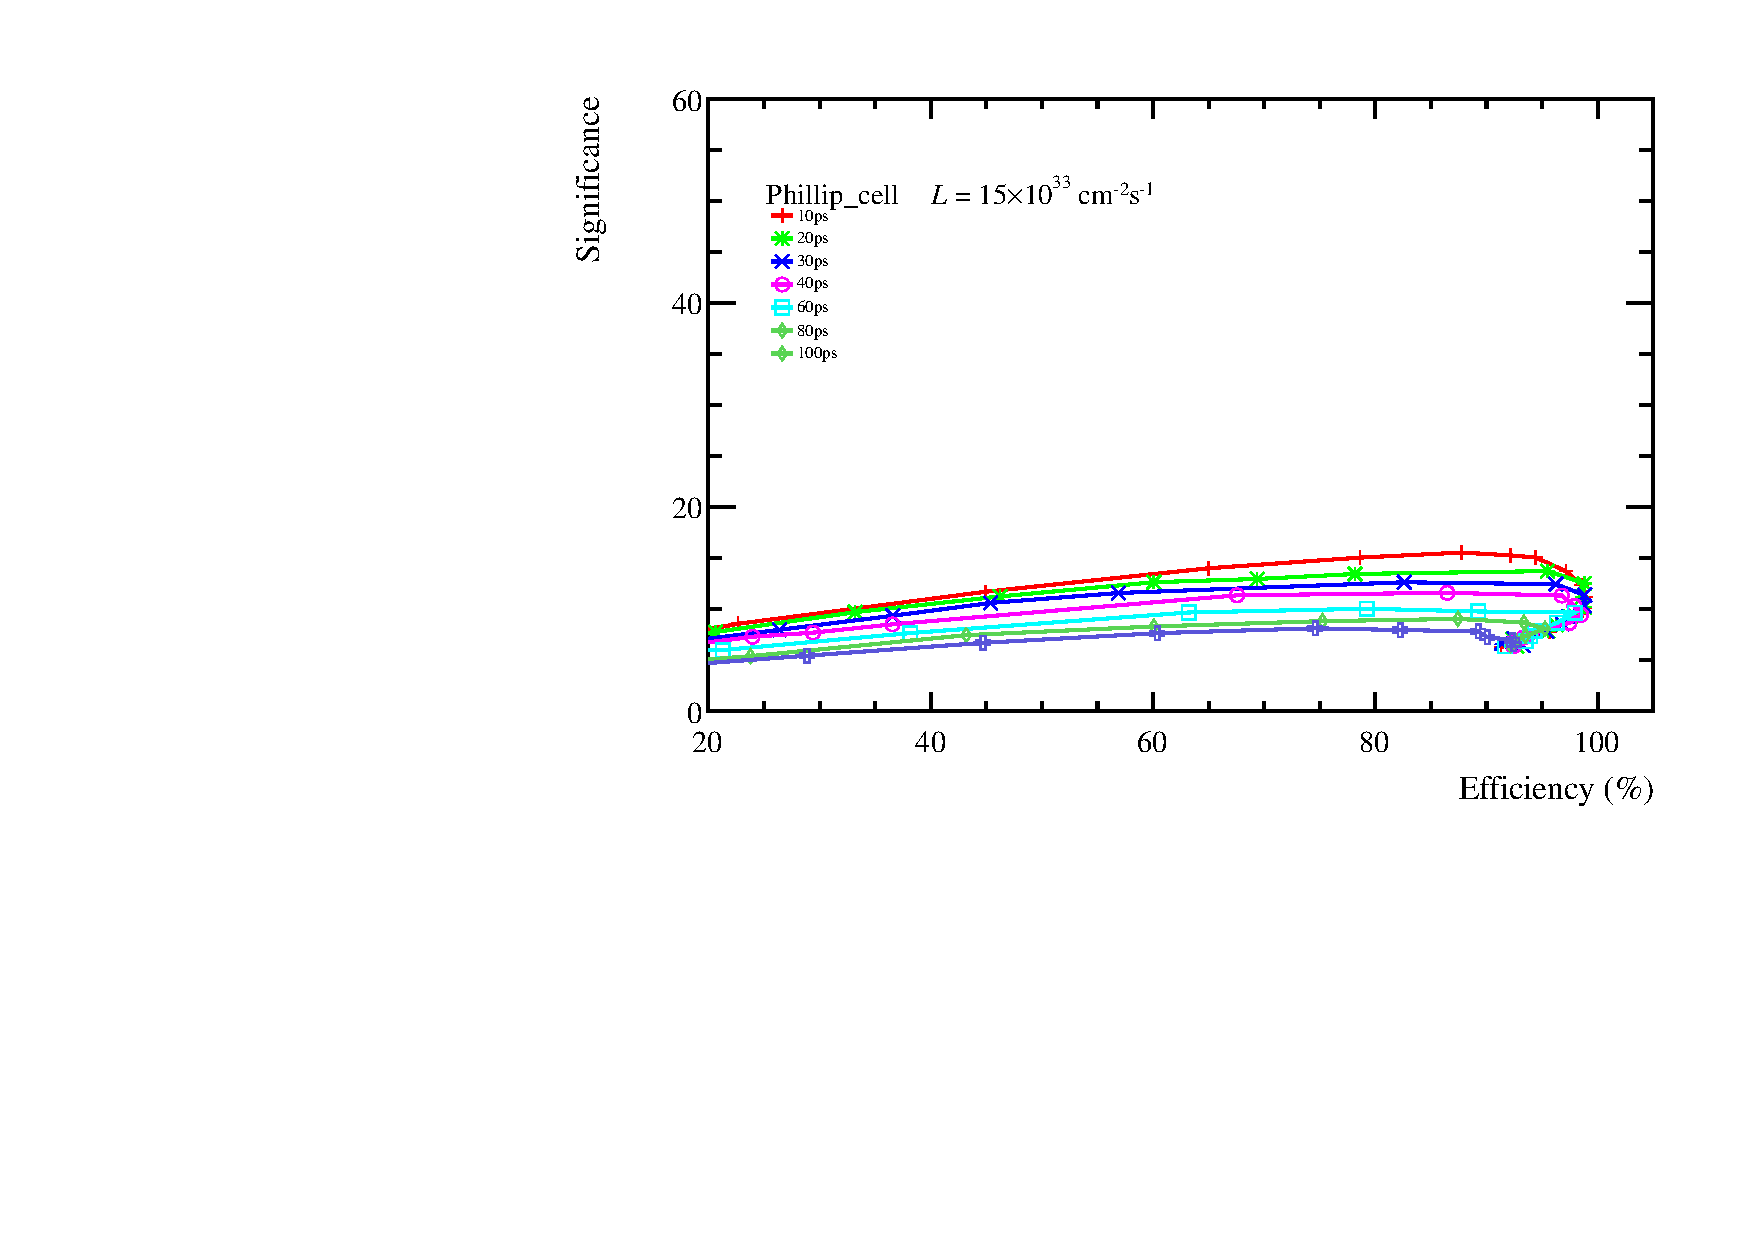
\includegraphics[width=0.45\linewidth]{Figures/06_ECAL/Fast_sim_Bs_JpsiPiz/eff_sig/Phillip_cell_Lumi_10_33_15_eff_signi.pdf}
    \\ 
    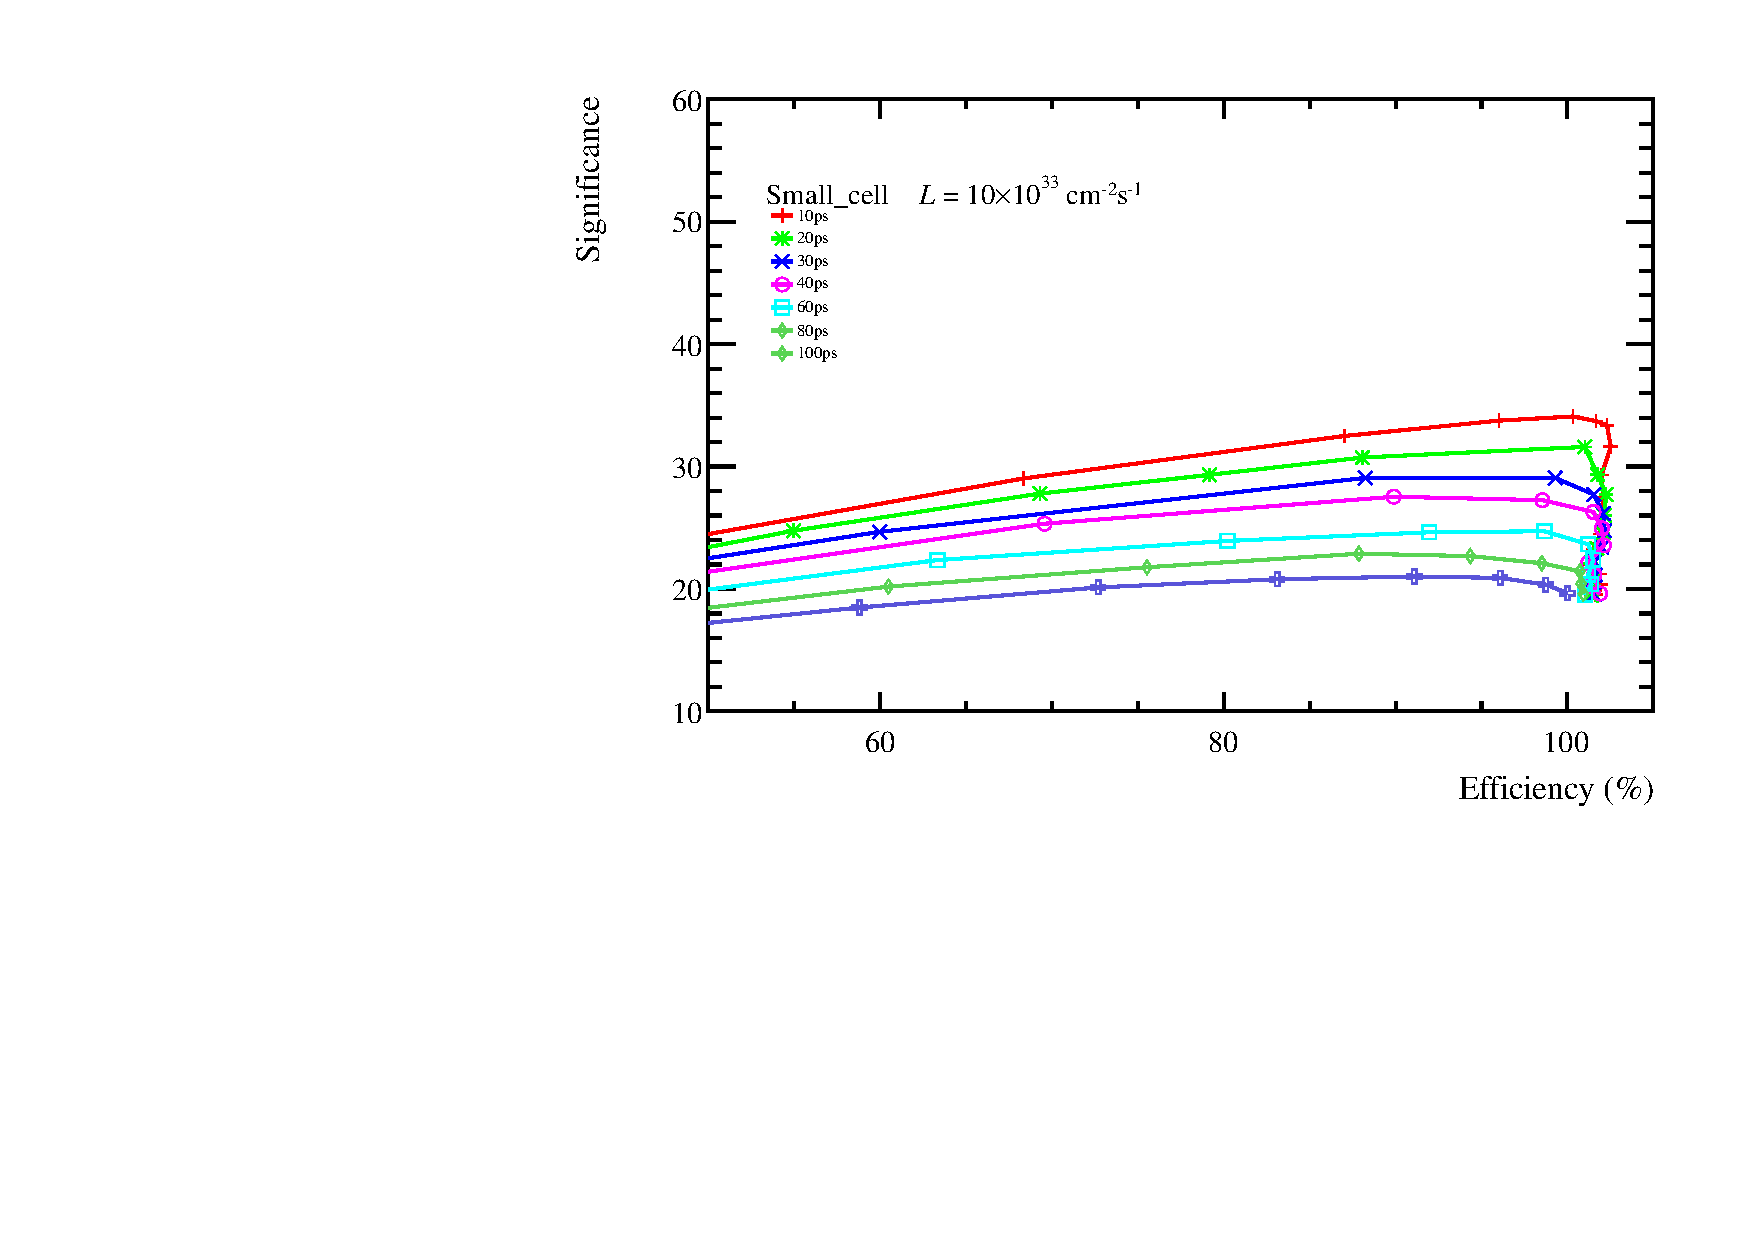
\includegraphics[width=0.45\linewidth]{Figures/06_ECAL/Fast_sim_Bs_JpsiPiz/eff_sig/Small_cell_Lumi_10_33_10_eff_signi.pdf} 
    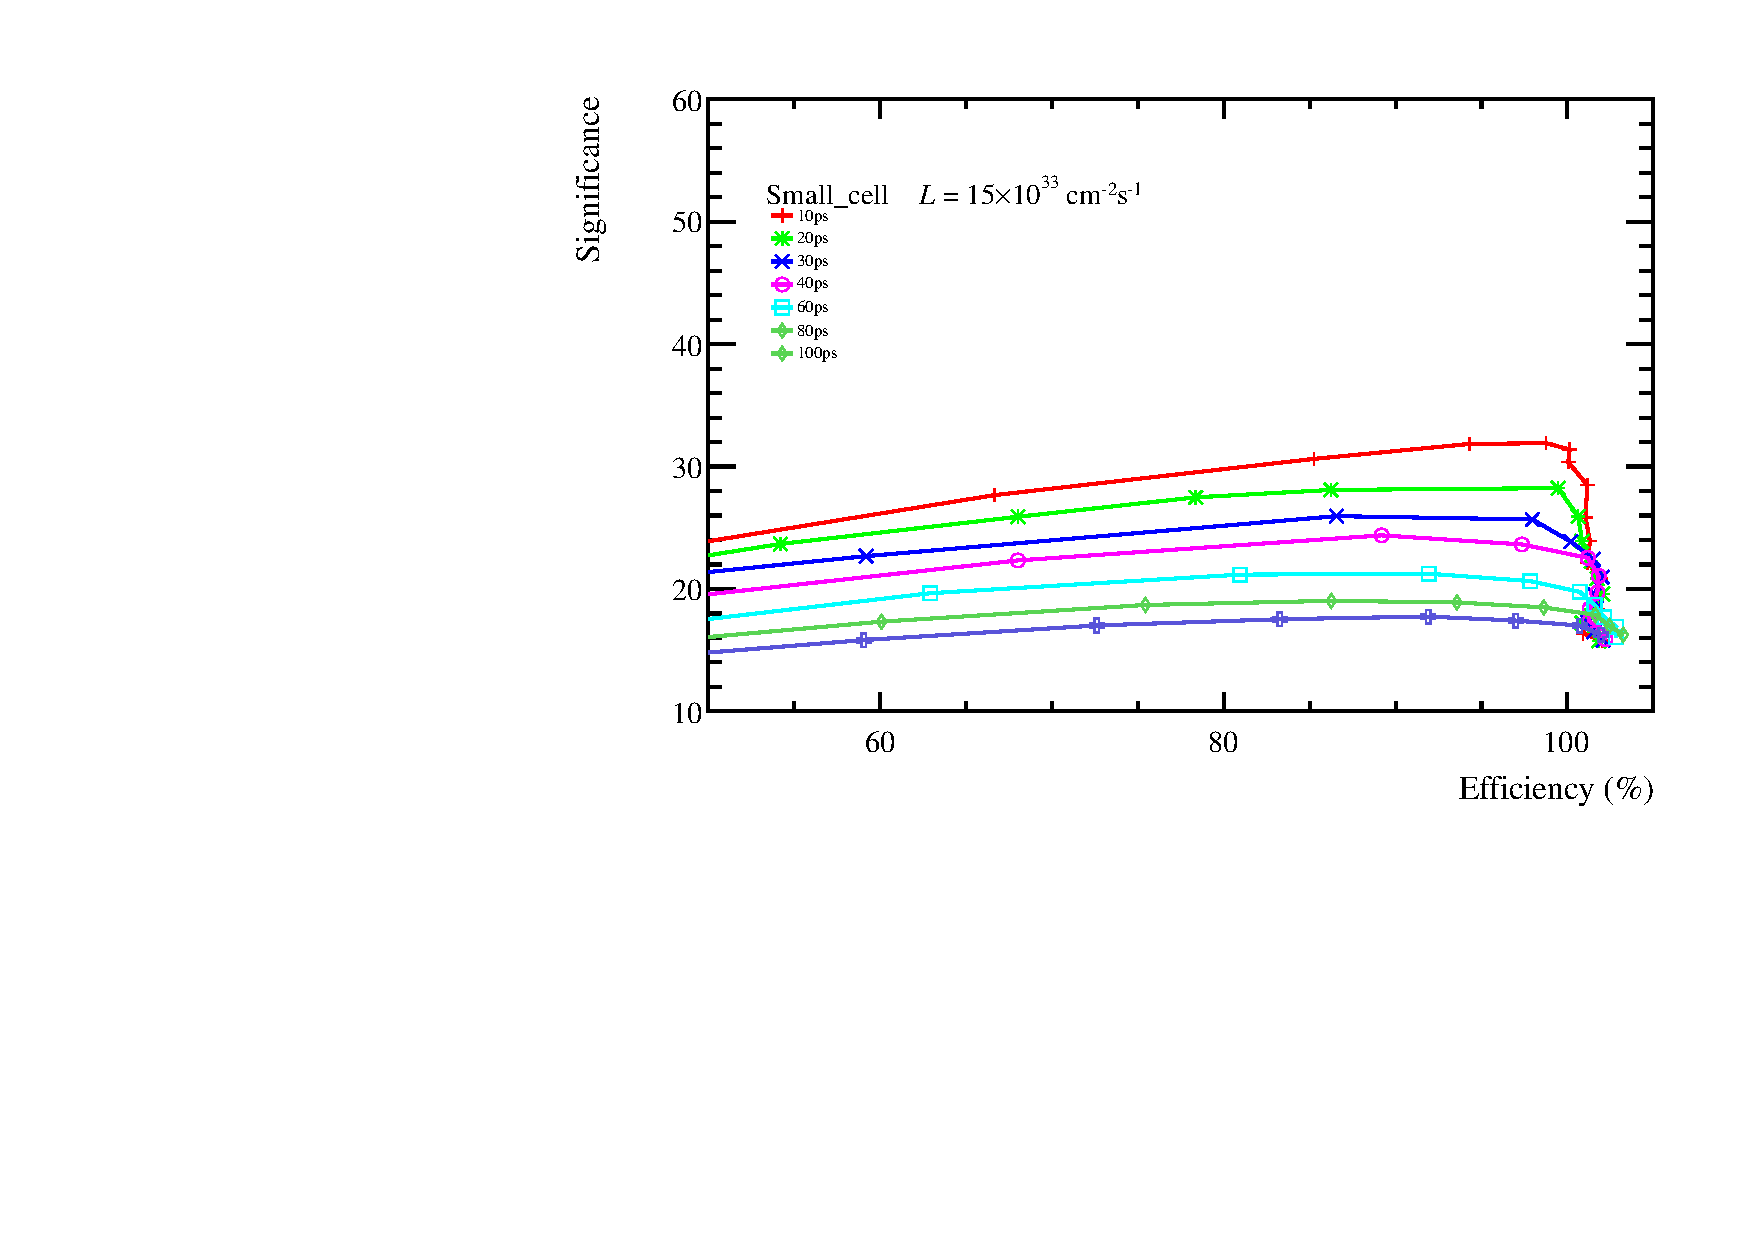
\includegraphics[width=0.45\linewidth]{Figures/06_ECAL/Fast_sim_Bs_JpsiPiz/eff_sig/Small_cell_Lumi_10_33_15_eff_signi.pdf}
    \\ 
    \vspace*{-0.5cm}
  \end{center}
  \caption{
     The relation between signal efficiency and significance with different $R(t)$ cuts applied,
   in Phillip's segmentation (top) and Si-W segmentation (bottom) respectively.
  }
  \label{fig:bs_Jpsipiz_phillip_eff_sig}
\end{figure}
%%%%%%%%%%%%%%%%%%%%%%%%%%%%%%%%%%%%%%%%


The performances of this additional selection value $R(t)$ in this decay channel is studied then.
The relation between selction efficiency and background rejection fraction after time matching applied with different time resolutions is shown in Figure.~\ref{fig:bs_Jpsipiz_phillip_eff_bkg}.
It is clearly that most of combinatorial background candidates can removed with the time resolution equal to tens of picosecond 
for both cell size segmentation.
The signel significance of $20000$ events simulation sample was also studied,
as shown in Figure.~\ref{fig:bs_Jpsipiz_phillip_eff_sig}.
When comparing the performances with different cell size segmentation,
the signal significance of Si-W \ecal improves a lot comparing to the Phillip's segmentation due to larger reconstruction efficiency.
It also means that smaller cell configuration can help improve the reconstruction efficiency of \piz.



\subsection{From parameterized simulation to \geant simulation}

From parameterized simualation,
we find that overlapping effect is the biggest challenge after \upgradetwo as high pile-up effet.
This causes a bad performance in the cluster reconstruction and particle identification.
Smaller cell size \ecal can recede this effect,
which leads to a better reconstruction effeciency and mass resolution in some physical channels.
Besides,
smaller cell size configuration can improve the reconstruction efficiency of resolved \piz,
which also results in a better mass resolution in the physical channel containing \piz.

In addition to smaller cell size,
timing information can also help eliminate high pile-up effect significantly.
On the one hand,
timing information can be used in the physical channel reconstruction,
the shower time should be coincident to the vertex time that the neutral particle decaying from,
a lot of combinatorial background candidates are removed by the timing matching.
On the other hand,
timing information can also be used in the cluster reconstruction and identification level,
help to identify the neutral particles from charged tracks by timing matching 
and removed random overlapping cluster effect according to the cell's time distribution in one cluster.
By studying the physical performance with different time resolution,
the timing resolution requirement for futher \ecal is around $~20 \ps$ for the particle with energy larger than $10 \gev$.

The technical proposal is not studied in the parameterized simualtion,
a possible technolgy chioce is using silicon sensor to measure shower time out of the experience of CMS,
which can meet the requirement to time resolution. 
In this next section,
we will discuss this performance of silicon-tungsten \ecal at \lhcb.
In the \geant model,
the idea by inserting several silicon layers to measure time in the shashlik or crystal \ecal is also discussed.




